%!TEX TS-program = xelatex
%!TEX encoding = UTF-8 Unicode

\documentclass{papon_thesis}
\usepackage{todonotes}
\usepackage{emptypage}

%\usepackage[]{showkeys}
\makeglossaries

\begin{document}
%\watermark {DRAFT COPY ONLY}
\newacronym{vos}{VOS}{Video Object Segmentation}
\newacronym{pdf}{PDF}{Probability Distribution Function}
\newacronym{mtt}{MTT}{Multi-Target Tracking}
\newacronym{ai}{AI}{Artificial Intelligence}
\newacronym{mtvt}{MTVT}{Multi-target visual tracking}
\newacronym{sbf}{SBF}{Sequential Bayesian Filtering}
\newacronym{msvs}{MSVS}{Mean-shift video segmentation}
\newacronym{mhvs}{MHVS}{Multiple hypothesis video segmentation}
\newacronym{pva}{PVA}{Propagation, validation, and aggregation}
\newacronym{pas}{PAS}{Predictive Association of Supervoxels}
\newacronym{vccs}{VCCS}{Voxel Cloud Connectivity Segmentation}
\newacronym{dof}{DoF}{Degree of Freedom}
\newacronym{dsst}{DSST}{Dynamic Semantic Segment Tracking}
\newacronym{lccp}{LCCP}{Locally Convex Connected Patches}
\newacronym{ddvg}{DDVG}{Depth Dependent Voxel Grid}
\newacronym{ecc}{ECC}{Extended Convexity Criterion}
\newacronym{vr}{VR}{Virtual Reality}
\newacronym{vsrtm}{VSRTM}{Video Segmentation by Relaxation of Tracked Masks}

% the front matter
% some details about the thesis
\title{Perceptual Parsing of Visual Streams through Hierarchical Tracking of Objects and their Parts}
\author{J\'{e}r\'{e}mie Papon}
\advisor{Prof. Dr. Florentin W\"org\"otter}

% about the degree
\degree{Doctor of Philosophy}
\field{Computer Science}
\degreeyear{2014}
\degreemonth{March}

% about the university
\department{Faculty of Natural Sciences and Mathematics}
\university{Georg-August-Universit\"{a}t G\"{o}ttingen}
\universitycity{G\"{o}ttingen}
\universitystate{Germany}

\makegermantitle
\cleardoublepage
\maketitle
\cleardoublepage
\pagenumbering{roman}\setcounter{page}{1}  
\referentpage
\newpage \thispagestyle{empty} \vspace*{\fill}
 
\noindent 

\textsc{  }
\begin{flushleft}
The canonical version of this document is the electronic copy maintained in the Github repository by the author. At this time, it is maintained at:\
\end{flushleft}
\begin{center} \url{https://github.com/jpapon/papon_thesis/thesis.pdf} \\ \end{center}

\begin{flushleft}
This work is licensed under a Creative Commons Attribution-NonCommercial 4.0 International License. The full terms of the license can be viewed online at:\
\end{flushleft}
\begin{center} \url{http://creativecommons.org/licenses/by-nc/4.0/} \\ \end{center}

\begin{flushleft}
Much of the code created as a result of the research in this thesis is freely available under a BSD license as part of the Point Cloud Library:\
\end{flushleft}
\begin{center} \url{http://www.pointclouds.org/} \\ \end{center}


\begin{flushleft}
The code for the Oculus Vision System (see Appendix \ref{chap:Oculus}) created as part of this thesis is freely available under GPLv3:\
\end{flushleft}
\begin{center} \url{https://launchpad.net/oculus} \\ \end{center}

\vspace{20pt}
\begin{center} For other usage, contact \url{jpapon@gmail.com}. \end{center}
\vspace{40pt}

\begin{center}
\begin{textsc}
\copyright~\textit{2014 \hspace{3pt}~- \theauthor} \\ 
\noindent All rights reserved.
\end{textsc}
\end{center}



\let\cleardoublepagecopy\cleardoublepage
\let\cleardoublepage\clearpage
\abstractpage
\tableofcontents
\listoffigures
\listoftables
\printglossary[type=\acronymtype,title=List of Acronyms,toctitle=Terms and Abbreviations]

\noindent
\begin{flushright}
\huge List of Related Publications
\end{flushright} 
\vspace{50pt} 

%The work described in this thesis has appeared in the following publications: \\
%\vspace{24pt} 

\hangindent=1.5cm Papon, J.;  Kulvicius, T.; Aksoy, E.; Wörgötter, F., ``\href{http://www.dpi.physik.uni-goettingen.de/cns/uploads_bibtexmodule/PDF/paponkulviciusaksoy2013.pdf}{Point Cloud Video Object Segmentation using a Persistent Supervoxel World-Model,}'' \emph{Intelligent Robots and Systems (IROS), 2013 IEEE/RSJ International Conference on}, Nov. 2013. \\
\vspace{12pt}

\hangindent=1.5cm Papon, J.;  Abramov, A.; Schoeler, M.; Wörgötter, F., ``\href{http://www.cv-foundation.org/openaccess/content_cvpr_2013/papers/Papon_Voxel_Cloud_Connectivity_2013_CVPR_paper.pdf}{Voxel Cloud Connectivity Segmentation - Supervoxels for Point Clouds,}'' \emph{Computer Vision and Pattern Recognition (CVPR) 2013}, June 2013. \\
\vspace{12pt}

\hangindent=1.5cm Papon, J.;  Abramov, A.; Wörgötter, F., ``\href{http://dx.doi.org/10.1007/978-3-642-33885-4_24}{Occlusion Handling in Video Segmentation via Predictive Feedback,}'' \emph{European Conference on Computer Vision (ECCV) 2012}. Workshops and Demonstrations, Lecture Notes in Computer Science Volume 7585, 2012, pp 233-242. \\
\vspace{12pt}

\hangindent=1.5cm Papon, J.;  Abramov, A.; Aksoy, E.; Wörgötter, F., ``\href{http://dx.doi.org/10.1109/WACV.2012.6163002}{A modular system architecture for online parallel vision pipelines,}'' \emph{Applications of Computer Vision (WACV) 2012}, pp.361-368, Jan. 2012. \\

\hangindent=1.5cm Stein, S.; Schoeler, M.; Papon, J.;  Wörgötter, F., ``{Object Partitioning using Local Convexity,}'' \emph{Computer Vision and Pattern Recognition (CVPR) 2013}, June 2014. \\

\hangindent=1.5cm Stein, S.;  Wörgötter, F.; Schoeler, M.; Papon, J.; Kulvicius, T., ``{Convexity Based Object Partitioning For Robot Applications,}'' \emph{Robotics and Automation (ICRA), 2014 IEEE/RSJ International Conference on}, June. 2014. \\

\vspace{100pt}

The research leading to this thesis was supported with funding from the European Community's Seventh Framework Programme FP7/2007-2013 (Specific Programme Cooperation, Theme 3, Information and Communication Technologies) under grant agreement no. 270273, Xperience and grant agreement no. 269959, Intellact.

 

\let\cleardoublepage\cleardoublepagecopy
\acknowledgments


\onehalfspacing
\mainmatter
% include each chapter...
\begin{savequote}[75mm]
Some Quote.
\qauthor{Quoteauthor Lastname}
\end{savequote}

%For an example of a full page figure, see Fig.~\ref{fig:myFullPageFigure}.

\chapter{Introduction}
\lettrine[lines=3, loversize=0.3]{\textcolor{DarkBlue}W}{hy are we here? What are we trying to do? Why bother?}
\todo[inline]{Motivation, put some applications}

\section{Problem Definition and Motivation}
This chapter presents the motivation behind our work by first discussing the three underlying problems that will be addressed throughout. To summarize into a brief statement, we would say our overall goal is the decomposition of video into semantically meaningful entities. That is, to move from the base \emph{low-level} pixels which compose an image to \emph{high-level} structures which are more representative of how a human would understand the scene. In the following sections we will introduce the three constituent underlying sub-problems: Image Segmentation, Multi-Target Tracking, and Video Object Segmentation.

\subsection{The Image Segmentation Problem}
Image segmentation aims to divide the set of pixels in an image into a number of distinct subsets, where each subset represents some semantically meaningful entity (e.g., an object - see Fig. \ref{fig:segmentation_example}). This is a notoriously tricky business, particularly because it is something that humans are able to do intuitively. This ease with which humans can segment visual scenes is highly deceptive; Marvin Minsky, one of the pioneers of Artificial Intelligence (AI), famously assigned one of his students ``computer vision'' as a summer undergraduate project in 1966. Nearly half a century later, despite the extensive effort to solve it, image segmentation, the first step on the long road to complete ``computer vision'', remains an unsolved problem. 

\todo[inline]{Some citations about image segmentation by humans (from CVPR paper)}
\begin{figure}
\label{fig:SegmentationExample}
\centering
\includegraphics[width=\linewidth]{figures/Introduction/segmentation_GT_example.png}
\caption[Example of Segmentation and Ground Truth]{Example of Segmentation and Ground Truth. From left to right we have an image, a segmentation from a computer vision algorithm, and a human-annotated ground truth labeling. Here labels are represented by different colors. We shall use this convention throughout the rest of this work.}
\end{figure}

The reason for this is two-fold: firstly, there are many technical or physical challenges associated with properly dividing an image into separate objects. Among these, shadows, occlusions, reflections, imaging noise and so forth can all greatly affect the results of image segmentation. Consider, for instance, a partial occlusion as in Fig. \ref{fig:SegmentationProblems}. A human can easily identify that the parts on either side of the occluder belong to same object. This is accomplished using what we shall refer to as \emph{high-level} knowledge throughout this work - in this case, knowledge of the complete nature of an object. 

This leads us to the second challenge in image segmentation, which is that, generally speaking, there is no ``correct'' solution to the problem. A perfect labeling for one application might be useless in another. This is even more of a problem when we are discussing segmentation separate from any application, as is the case with standard image segmentation benchmarks (which are use to quantify algorithm performance). These benchmarks use ground-truth image labels (manually created by humans) to score the output of different algorithms. Unfortunately, the correctness of different labelings is highly subjective, and hand-drawn labels from  people can differ radically.

\begin{figure}
\label{fig:SegmentationProblems}
\centering
\includegraphics[width=\linewidth]{figures/Introduction/Segmentation_Problems.pdf}
\caption[Technical Difficulties of Segmentation]{Technical Difficulties of Segmentation. Here we see some of the myriad of technical difficulties present in color-based segmentation, such as transparent objects (the water bottle), partial occlusions (the toaster), objects with strong color differences (the little monster), and similarities in color (the bottle cap to the table).}
\end{figure}


\subsection{The Tracking Problem}
Multi-target visual tracking (MTVT) is a crucial challenge for many computer vision applications such as visual surveillance, action recognition, and robotic imitation learning. In many such functions, visual tracking serves as the precursor to all further high-level inference, making robust tracking fundamental to the success of a large variety of intelligent systems. The general goal of MTVT is to sequentially estimate the number of targets and their corresponding states (e.g., position, velocity). This is accomplished by associating noisy observations over time with the entities which produced them. Tracking links targets into sequential states (known as \emph{tracks}), typically using some a-priori detection model, such as tracking a human face in video based on a facial model. In general, this is done by estimating some state for each tracked object (e.g. a bounding box around a person's face) given an observation (e.g., the output of a face detector).

\begin{figure}
\label{fig:ExampleTracking}
\centering
\includegraphics[width=\linewidth]{figures/Introduction/Tracking_Example.pdf}
\caption[Example of Visual Tracking]{Example of Visual Tracking. This shows outputs from various trackers in a standard video tracking benchmark. Some of the difficulties of tracking can be seen- in particular complex backgrounds, motion blur, partial occlusions (second frame from left) and even full occlusions (right-most frame).}
\end{figure}

The primary challenge in MTVT is the data association problem - deciding which tracked target a particular observation belongs to. Confounding this is the additional null possibility, where an observation belongs to none of the tracked targets. Closer examination reveals that the difficulties are related to those of image segmentation, simply extended into the temporal dimension. In particular, interacting and occluded targets are especially challenging.

\subsection{Video Object Segmentation - Segmentation In Sequential Frames}
Video object segmentation (VOS) attempts to cluster pixels of video frames into segments which are both spatially and temporally coherent. While similar to MTVT, VOS goes a step beyond localizing tracked objects, in that it makes an association decision for each observed pixel; in addition to estimating overall state, it must re-estimate spatial extent every frame. Additionally, VOS has the additional consideration that target appearance models are unknown a-priori, and are subject to arbitrary changes over time. 

\begin{figure}
\label{fig:ExampleSegmentation}
\centering
\includegraphics[width=\linewidth]{figures/Introduction/Video_Segmentation.pdf}
\caption[Example of Video Object Segmentation]{Example of Video Object Segmentation - from \cite{Abramov_WACV12}. This shows the goal of VOS - to extract a dense labeling (labels here are shown as distinct colors) for every frame, maintaining temporal consistency of objects. For many applications it is of vital importance to make the labeling consistent from frame to frame, that is, to maintain object identities.}
\end{figure}

One interesting aspect of video segmentation is that it has the potential to be more accurate than single image segmentation, as it can take advantage of the temporal coherence of objects to infer information about the objects in a scene. Unfortunately, the addition of the temporal domain brings along new challenges as well; for instance that pixels which should be grouped across time may not be continuously visible, as in the case of partial or full occlusions. Additionally, the added dimension increases the computational complexity of the problem, making accurate segmentation a costly procedure. Temporal information also increases the exposure of the algorithm to noise, as each image frame is a separate noisy measurement. This adds a large amount of uncertainty to the problem, since measured values (i.e., of color) for an object can show significant variation over time. 
 
\section{State of the Art}
\subsection{Segmentation and Superpixels}
Segmentation of scenes into objects remains one of the most challenging topics of computer vision despite decades of research. To address this, recent methods often use hierarchies which create a rank order that build bottom-up from small localized superpixels to large-scale regions \cite{Ren:ICCV2003,Ahuja:CVPR2008,Arbelaez:PAMI2011}. As an alternative, researchers have also pursued strictly top-down approaches. Such methods began with coarse segmentations using multiscale sliding window detectors \cite{ViolaJones:IJCV2004}, later progressing to finer grained segmentations and detections based on object parts \cite{Felzenswalb:PAMI2010, Bourdev:ICCV2009}. These two avenues of research led naturally to methods which {\em combine} bottom-up hierarchy building with top-down object- and part-detectors \cite{Arbelaez:CVPR2012, Silberman:ECCV12, Gupta:CVPR2013}. While these approaches have yielded quite good results even on complex, varied data sets, they have lost much of the generality of learning-free approaches. In general the most powerful methods to-date use trained classifiers for segmentation \cite{Silberman:ECCV12, Gupta:CVPR2013}. This means they cannot be applied to arbitrary unknown scenes without being retrained, requiring the acquisition of a new data-set tailored to each test environment.

\subsection{Multi-Target Visual Tracking}
Multi-Target Visual Tracking is a well-established field, which goes back over thirty years \cite{MTT_JPDA}. In this work we use Sequential Bayesian Filtering (SBF), a technique which recursively estimates the time-changing posterior distribution of target states given all previous observations. We use a Sequential Monte Carlo method known as Particle Filtering to approximate the posterior, an approach which was first introduced to the vision community by Isard and Blake \cite{Condensation98} and has been the subject of much subsequent research extending it to multiple targets \cite{TrackingMultipleParticleFiltering,MonteCarloMTT,SequentialMonteCarloMultitargetFiltering}. For details on how one approximates SBF using a Particle Filter we refer the reader to Appendix B.

Initially, researchers pursued two avenues of research in extending a single Particle Filter to multiple targets. The first was to represent all targets jointly in a single particle filter by assigning individual particles to particular labels \cite{MultiMixtureTracking03}. This means that, for a given total number of particles, there will be fewer for each individual target - resulting in reduced accuracy. The second approach was to add additional dimensions to the state space for each additional target \cite{TrackMultTargets01}. Unfortunately, this approach quickly increases the dimensionality of the state space, resulting in a need for a very high number of particles for the filter to remain accurate. In both approaches, the computational complexity increases exponentially as targets are added (for constant level of accuracy), as both seek to find a joint solution. As a consequence of this, it is beneficial to use a separate particle filter for each target. One way of doing this is to add factors to the observation and/or process models of the filters which explicitly model occlusions and interactions between targets \cite{MCMCParteFilt_05, ApproxMultiTrack_06}. 

Another approach which has generated much interest is to use the output of detectors as the basis for tracking. Known as \emph{tracking-by-detection}, these methods typically use independent particle filters to maintain tracks \cite{RobustVTMT_06,MultipersonTBD_011}, and place the focus of the problem on the data association step, wherein detections are assigned to targets. While there are several classical approaches for solving this association problem from Sonar and Radar research \cite{SonarMultiTrack_83,MultiTrack_79}, a greedy approach is typically sufficient given a good association scoring function \cite{DetTrackMultiHumans_07,MultipersonTBD_011}. 
%%%%%%%%%%%%
%Good review in - Detection and Tracking of Multiple, Partially Occluded Humans by Bayesian Combination of Edgelet based Part Detectors
%%%%%%%%%%%%%%%%%%%%%%%%%%%%

\subsection{Video Object Segmentation}
There are many existing video object segmentation (VOS) methods, which can be classified based on three parameters; whether they are on- or off-line, whether they are dense or sparse, and whether or not they are supervised. We can reduce the comparison-space of related work by comparing only with algorithms which have the same three parameters as this work - on-line processing (the algorithm may only use past data), dense segmentation (every pixel is assigned to a spatio-temporal cluster), and unsupervised operation. Four state-of-the-art segmentation algorithms meet these requirements: Mean-shift video segmentation (MSVS) \cite{MSVS}, Multiple hypothesis video segmentation (MHVS) from superpixel flows \cite{MHVS}, Propagation, validation, and aggregation (PVA) of a preceding graph \cite{PropValAgg}, and Matching images under unstable segmentations \cite{MatchingUnstable}.  Of these methods, none are able to handle full occlusions; in fact only MHVS considers occlusions, and it is only able to handle partial 
occlusions for a few frames, and does not consider full occlusions. Even state of the art off-line methods such as that of Brendel and Todorovic \cite{SegTrackRegions} only handle partial occlusions, claiming that ``complete occlusions ... require higher-level reasoning''.  

Multiple hypothesis video segmentation (MHVS) from superpixel flows \cite{MHVS} provides dense online unsupervised video segmentations, but is only able to handle partial occlusions for a few frames, and does not consider full occlusions. There also has been much recent work in VOS specifically addressing the problem of segmenting foreground from background \cite{MWCwMC,GC_SURF}. While these works have been to shown to perform very well in their task, they only solve the single target case, as they do not need to resolve the multiple association problem.

In \cite{TrackingOcclusionsGraphCuts} Papadakis and Bugeau use a dynamical model to guide successive segmentations, along with an energy function minimized using graph cuts to solve the label association problem. They formally model visible and occluded regions of tracked objects, tracking them as distinct parts. While they do consider occlusions, they do not maintain a world model, and as such their methodology must fail under complete occlusions.  Additionally, they formally model visible and occluded parts of the tracked objects, and so the method does not scale well with an increasing number of objects, and thus is better suited to extracting the silhouettes of a few objects than performing a full segmentation. Other methods, such as \cite{LayeredGraphicalModels}, are severely limited in that they require pre-
computed models which are calibrated to a ground plane in order to resolve occlusions. Recent work in MTVT~\cite{MultiObjectTracking} successfully tracks multiple objects using a segmentation and association approach and adaptive 3D appearance models, but is limited by the need to align model point clouds to the observed data every frame, as well as the need for a ground plane. This precludes it from handling occlusions, as once a target is no longer observed, its track must be terminated.

\section{Outline and Contributions}

This thesis is organized as follows: First, in Chapter \ref{Chap:VideoSegRelaxation} we present a hybrid Video Object Segmentation / Multi-Target Tracking technique for 2D data. We describe the method, briefly describe the segmentation algorithm it relies on, and present results on a tracking benchmark. In Chapter \ref{Chap:WorldModel} we present the concept of a persistent 3D voxel world model. We begin by briefly introducing some core concepts of acquisition and representation of 3D pointcloud data, then present Voxel Cloud Connectivity Segmentation (VCCS), a method for extracting a graph of 3D voxel patches from pointcloud data. We then discuss how to add pointclouds sequentially to the model in a way that allows voxels to persist through occlusions. In Chapter \ref{Chap:ModelBasedTracking} we describe a method for using particle filters to track multiple rigid objects in pointcloud video data and present results of tracking performance on artificial data. In Chapter \ref{Chap:TrackingBasedSegmentation} we combine the methods described in prior Chapters into a system which can produce full video segmentation of pointcloud videos. We show that the system is highly robust to occlusions and noisy data, and give results for the application of semantic understanding of human actions. Finally, in Chapter \ref{Chap:Conclusions} we discuss the findings and experimental results of this work, possible future work, and conclude.

Each of the Chapters in this thesis contain novel contributions to the field: 
\todo[inline] Add citations for these to relevant papers
\begin{itemize}
\item {\bf Chapter \ref{Chap:VideoSegRelaxation} } contains the 2D segmentation through relaxation technique. 

\item {\bf Chapter \ref{Chap:WorldModel} } contains the Supervoxel clustering method, as well as the scheme for maintain voxels in an Octree through occlusions. 

\item {\bf Chapter \ref{Chap:ModelBasedTracking} } has the scheme for accelerating 3D particle filter tracking through stratified sampling of the model-space. 

\item {\bf Chapter \ref{Chap:TrackingBasedSegmentation} } has the techniques used to generate full segmentations based upon the results from multiple independent trackers. Additionally, Appendix A presents the Oculus Vision System, a computer vision system created over the course of the research for this thesis.
\end{itemize}
\cleardoublepage
\cleardoublepage
\begin{savequote}[75mm]
Some Quote.
\qauthor{Quoteauthor Lastname}
\end{savequote}

%For an example of a full page figure, see Fig.~\ref{fig:myFullPageFigure}.

\chapter{Video Segmentation by Relaxation of Tracked Masks}
\label{Chap:VideoSegRelaxation}
\lettrine[lines=3, loversize=0.3]{\textcolor{DarkBlue}I}{n the beginning}, 3D data, especially video data, was not readily available. As such, researchers were forced to make due with strictly 2D video, which is inherently ambiguous in many situations. In particular, partial and full occlusions are particularly vexing problems in 2D video - not least because understanding of 2D video is so easy for humans, yet so difficult to interpret algorithmically. Indeed, knowledge of object permanence, that is, the understanding of how to correctly interpret occlusions, is something that humans acquire very early on in their lives \cite{ObjectPermanence}, but has yet to be successfully implemented in a fully automated \gls{vos} system. Even after decades of research, state-of-the-art methods still have trouble correctly resolving partial occlusions, and typically fail completely after even the briefest of complete occlusions.

In this Chapter, we shall present our attempts towards resolving the object permanence problem with 2D data, as well as advance color-based \gls{vos} in general. In particular, we seek to overcome two of the main drawbacks of the color-based video segmentation method developed by Abramov et al. \cite{Abramov_RealtimeSegmentation} (and indeed, of color-based \gls{vos} in general). The first of these is the correct tracking of objects through partial and full occlusions, which we proposed to solve using a layering of deformable object masks that are allowed to interact and compete for ``ownership'' of pixels. The second is to allow for object identities to be maintained through sudden and/or fast movements - something that was not possible due to the core assumptions of the algorithm. To correct for this, we tracked the masks with a set of particle filters, a class of Bayesian predictive filters which are well known for their ability to handle difficult trajectories \cite{TrackingMultipleParticleFiltering,MonteCarloMTT,SequentialMonteCarloMultitargetFiltering}.

The underlying principle guiding the proposed algorithm is to use predictions from Bayesian filtering to inform segmentation of higher-level temporal object correspondences. It is well known that sequential Bayesian estimation methods perform well in difficult tracking scenarios \cite{Doucet2001}, and, under the Markov assumption, are computationally less demanding than video segmentation techniques such as MHVS \cite{MHVS}, which consider many prior frames. Particle filtering is one such method which has been shown to approximate the optimal tracking solution well, even in complex multi-target scenarios with strong nonlinearities \cite{TrackingMultipleParticleFiltering,MonteCarloMTT,SequentialMonteCarloMultitargetFiltering}. 

\section{Overview of the Algorithm}
\label{sec:Overview}
Before proceeding to discuss elements in detail, we shall first give a brief overview of the algorithm (depicted in Figure \ref{fig:AlgorithmFlow}). We begin by performing an initial segmentation (using any method) on the first frame $\mathbf{F}_{t_0}$ to generate an initial set of labels $\mathbf{S}_{t_0}$. An initial set of particles is generated for each label, and color histogram features are computed for each particle (as in \cite{ColorBasedProbabilisticTracking}). Thus each object $k$ at initial time $t_0$ is specified by a set of $N_k$ particles $\mathbf{X}^{k,1:N_k}_{t_0}$, each of which contains a representation of the object, specified by a pixel existence map $\mathbf{M}$, a reference color histogram $\mathit{\hat{q}}$, a position shift vector $\mathbf{p_{t_0}}$, and a velocity vector $\mathbf{v_{t_0}}$.

\begin{figure}
\includegraphics[width=\linewidth]{figures/ECCV2012/AlgorithmFlow2.pdf}
  \caption[Overview of Algorithm]{Flow of algorithm for one time step, shown for three labels ($k_1$, $k_2$, and $k_3$). For a description, see Section~\ref{sec:Overview}.}
\label{fig:AlgorithmFlow}
\end{figure}

The particles are then propagated in time independently, shifting their existence maps to new regions of the image. These shifted maps are used to generate measured color histograms from the next frame, which are evaluated to determine similarity to the object's reference histogram. The set of particles for each object is then combined to create an overall object pixel likelihood map. The pixel likelihood maps for all objects are then further combined with each other to create a label association likelihood map. In this likelihood map, each pixel is a \gls{pdf} specifying the probability that the original image pixel was generated from an observation of a particular object.

The label association likelihood map is then sampled using a per-pixel selection procedure (as described in Section~\ref{sec:LabelAssocLikelihoodMap}) to generate a candidate label image, $\tilde{\mathbf{S}}_{t_0+1}$. This candidate image is used as the initialization for the Metropolis-Hastings algorithm with annealing of Abramov et al. \cite{Abramov_RealtimeSegmentation}, which updates the labels iteratively until an equilibrium segmented state is reached. The segmentation result, $\mathbf{S}_{t_0+1}$  is subsequently used to update the set of particles via three mechanisms; birth, decay, and repopulation. Birth is used for new labels in the segmentation output, and consists of initializing a new set of particles. Decay occurs when a label is not found in the segmentation output, and consists of killing a number of the particles of the missing label. The most commonly occurring mechanism, repopulation, occurs for all previously existing object labels which are found. Repopulation rejuvenates the set of particles for an object by replacing a number of particles in the set with new particles based on the relaxed segmentation result. 

\section{Tracking Object Masks}
We shall now describe each of the parts of the algorithm given above in further detail, beginning with a description of how we track object masks using particle filters. First we will briefly review the basic principles of sequential Bayesian estimation and particle filtering, and then show how they can be used to predict pixel-level label associations in order to seed a segmentation algorithm.

\subsection{Sequential Bayesian Estimation}
Sequential Bayesian estimation uses a state space representation, in which a state vector $\mathbf{x}_t$ describes the hidden state of a dynamic system. Bayesian estimation attempts to determine the posterior distribution of the state given all prior observations $\mathbf{z}$, i.e., $\mathit{p}(\mathbf{x}_t|\mathbf{z}_{1:t})$. This is accomplished using a two step recursion which first generates a hypothesis of the current state conditioned on the previous state and then performs a Bayes update using the new observation. These steps are known as the prediction and filtering steps, respectively. 

The prediction step estimates the current distribution given all prior observations, or
\begin{equation} \label{eqn:prior}
\mathit{p}(\mathbf{x}_t|\mathbf{z}_{1:t-1}) =  \int{ \mathit{p}(\mathbf{x}_t|\mathbf{x}_{t-1})\mathit{p}(\mathbf{x}_{t-1}|\mathbf{z}_{1:t-1}) \mathit{d}\mathbf{x}_{t-1}}. 
\end{equation}
This prediction requires the specification of a stochastic \textit{dynamic model} 
\begin{equation} 
\mathbf{x}_t = \mathit{f}_t(\mathbf{x}_{t-1},\mathbf{v}_t) ,
\end{equation}
where $\mathbf{v}_t$ is the process noise, which characterizes the state transition density $\mathit{p}(\mathbf{x}_t|\mathbf{x}_{t-1})$. The dynamic model takes advantage of knowledge of the system to generate reliable predictions of how the state evolves. 

The filtering step uses Bayes rule to update the predicted density by conditioning it on the new observation $\mathbf{z}_t$:
\begin{equation} \label{eqn:posterior}
\mathit{p}(\mathbf{x}_t|\mathbf{z}_{1:t}) =  \frac{ \mathit{p}(\mathbf{z}_t|\mathbf{x}_{t})\mathit{p}(\mathbf{x}_{t}|\mathbf{z}_{1:t-1})} {\mathit{p}(\mathbf{z}_{t}|\mathbf{z}_{1:t-1})}. 
\end{equation}
This requires the specification of an observation, or measurement, model
\begin{equation} 
\mathbf{z}_t = \mathit{h}_t(\mathbf{x}_{t},\mathbf{w}_t) ,
\end{equation}
where $\mathbf{w}_t$ is the measurement noise, which characterizes the observation density $\mathit{p}(\mathbf{z}_t|\mathbf{x}_{t})$. Once the filtered, or posterior distribution is determined, an estimate of the state can be made using a variety of techniques (e.g., maximum a-posteriori, mean-shift). 

\subsubsection{Dynamic Model}
In our method, the state of a particle consists of four elements; the pixel existence map $\mathbf{M}$, a reference color histogram $\hat{q}$, a position shift vector $\mathbf{p}$, and a velocity vector $\mathbf{v}_t$. Of these, only the position shift and velocity evolve over time, so we adopt the state vector
 \begin{equation} 
 \mathbf{x}_t = [p_x v_x p_y v_y]^T ,
 \end{equation}
where $(p_x,p_y)$ denotes the accumulated shift of the pixel existence map in the image plane, and $(v_x,v_y)$ the map velocity in the image plane. Motion is modeled using a constant velocity model in discrete time with uniform sampling period $\mathit{T}$, giving the dynamic model
\begin{equation} \mathbf{x}_t = \mathbf{A}\mathbf{x}_{t-1} + \mathbf{v}_t , \end{equation}
where
\begin{equation} \mathbf{A} = 
\begin{bmatrix}
 1 & \mathit{T} & 0  & 0 \\ 
 0 & 1 & 0 & 0\\ 
 0 & 0 & 1 & \mathit{T}\\ 
 0 & 0 & 0 & 1
\end{bmatrix} \end{equation}
and noise $\mathbf{v}_t$ is assumed to be zero mean Gaussian with fixed covariance.

\subsubsection{Measurement Model}
In our method measurements are taken by calculating a color histogram, $\mathit{q}_t$ for the region lying within the shifted pixel existence map $\mathbf{M}$. That is, for particle $n$ of object $k$,
\begin{equation}
\mathit{q}^{k,n}_t = hist( \mathbf{F}_{t} \cap \mathbf{M}^{k,n}_t ).
\end{equation}
Color histograms are three dimensional, with 8 bins for each of the color components hue, saturation, and value. As in \cite{ColorBasedProbabilisticTracking}, a Gaussian density is used for the observation density $\mathit{p}(\mathbf{z}_t|\mathbf{x}_{t})$, that is
\begin{equation} 
\label{eqn:Weighting}
\mathit{p}(\mathbf{z}_t|\mathbf{x}_{t}) = \frac{1}{\sqrt{2\pi}\sigma} \exp{-\frac{\Delta(\hat{\mathit{q}},\mathit{q}_t)^2}{2\sigma^2}}, 
\end{equation}
where $\Delta(\mathit{\hat{q}},\mathit{q}_t)$ is the Bhattacharyya distance (as proposed in \cite{Real-timeTrackingMeanShift}) between the reference histogram $\mathit{\hat{q}}$ for the particle and the measured histogram $\mathit{q}_t$ for time $\mathit{t}$. The Bhattacharyya distance is a standard measure of similarity between discrete probability distributions, and is defined as
\begin{equation} \Delta(\hat{\mathit{q}},\mathit{q}_t) = \sqrt{1- \sum{\sqrt{\hat{\mathit{q}}\mathit{q}_t }}}. \end{equation}

\subsection{Parallel Particle Filters}
Except in special cases (e.g., Kalman Filter), closed-form solutions to Equations \eqref{eqn:prior} and \eqref{eqn:posterior} are not available. Particle Filters are a Monte-Carlo method designed to approximate the posterior distribution with a weighted set of random samples. There are many excellent descriptions of the mechanics of particle filtering available (such as \cite{Doucet2001}), so we shall avoid presenting them here, and proceed directly to presenting the details of our algorithm. 

The predictive portion of the method uses multiple Sequential Importance Resampling (SIR) filters in parallel to track multiple targets (labels) simultaneously. At this stage in the algorithm targets are assumed independent and interaction between labels is therefore not considered (interaction is accounted for later, as described in Section \ref{sec:Label Image Generation}). Particles are first propagated using the constant velocity dynamics model, and their predicted existence maps $\tilde{\mathbf{M}}^{k,n}$ are used to generate a measured histogram, $\mathit{q}_t$. Particles are weighted based on \eqref{eqn:Weighting}, and then normalized as a set for each label $k$. Systematic resampling is used to prevent particle degeneracy, due to its speed and good empirical performance \cite{Doucet2001}.

The resulting distributions from the weighting procedure are used to generate object pixel likelihood maps for each label,$\hat{\mathbf{M}}^{k}_{t+1}$, which are then combined into the label association likelihood map $\hat{\mathbf{L}}_t$, as described in Section \ref{sec:Label Image Generation}. A realization of this likelihood map can then be relaxed to produce a final segmented output, $\mathbf{S}_t$. 

\subsection{Particle Birth, Repopulation, \& Decay.}
One key improvement of the proposed algorithm over prior particle filtering methods is its use of the segmentation result $\mathbf{S}_{t}$ to update the particle sets. This allows the creation of new targets, adaptation to changing target appearance, and gradual elimination of targets which are no longer observed. This is accomplished via three mechanisms, which we term, respectively, birth, repopulation, and decay. 

Birth occurs when a label which has not existed previously is found in the segmentation output $\mathbf{S}_{t}$, or more formally $ \{ k\notin \mathbf{S}_{1:t-1}, k\in \mathbf{S}_{t}\}$. It consists of generating a set of particles $\mathbf{X}^k$ for the new label using $\mathbf{S}_{t}$ to initialize an existence map $\mathbf{M}^k_t$ and $\{\mathbf{F}_{t} \cap \mathbf{M}^k_t \}$ to calculate a reference color histogram $\hat{\mathit{q}^k_t}$.

Repopulation is a key component of the algorithm, as it allows the pixel likelihood map for an object, $\mathbf{\hat{M}}^k$, to adapt over time to the changing appearance of the object. Every iteration, all previously existing object labels which are found in $\mathbf{S}_{t}$ are repopulated by replacing some particles in the set with particles generated from $\mathbf{S}_{t}$ and $\mathbf{F}_{t}$. Particles are chosen for replacement using stratified sampling, at a rate specified by parameter $\lambda_r$. The repopulation mechanism gradually modifies the object "model" through the addition of particles which have an updated existence map and color histogram (coming from the segmentation result). We use the term model here loosely, since there is in actuality no explicit model for any of the objects - merely a pixel likelihood map generated at each time step from the objects constituent particles and the current image frame. 

Stratified replacement and relatively low repopulation rates are used to help keep the influence of erroneous hypotheses to a minimum, but as with any adaptive method, they can occasionally lead the tracker astray. Replacement of particles, rather than updating of a central model, helps to reduce this problem, since a few erroneous particles will generally not completely derail the algorithm. Nevertheless, future work could investigate strategies that allow pruning of unlikely hypotheses without negatively affecting occlusion handling. 

Decay occurs when a label is not found in the segmentation output, $ k \notin \mathbf{S}_t $. Particles are selected from $k$ using random sampling, at a rate determined by the decay rate $\lambda_d$, and are pruned; they are no longer considered when filtering $k$. This reduces the number of active particles for the label in the next iteration, $N^k_{t+1}$, by approximately $\lambda_d N^k_t$. If the number of active particles for a label falls below a certain threshold, $N_{min}$, then the set of particles for the label is deleted, and the object is no longer tracked. If a label which was being decayed is observed again, i.e., $ \{ k\notin \mathbf{S}_{t-1}, k\in \mathbf{S}_{t}\}$, then the label is revived by replacing particles which had been killed with new particles, which are initialized as in the repopulation step.

\section{Extracting a Dense Image Labeling}
\label{sec:Label Image Generation}

The middle portion of Figure \ref{fig:AlgorithmFlow} depicts how the candidate label image,  $\tilde{\mathbf{S}}_{t}$, is generated. The candidate label image is a summary of the accumulated knowledge of the particle filters; it is a prediction of what the segmented scene should look like. That is to say, it is a pixel-wise realization of the label association likelihood map $\hat{\mathbf{L}}_{t}$, which is constructed by combining the object pixel likelihood maps (which approximate the posteriors of the particle sets). $\tilde{\mathbf{S}}_{t}$ is the seed of the segmentation kernel, which uses pixel values from $\mathbf{F}_t$  to perform the relaxation process and generate a dense label image. In this section we will describe the process of generating the object pixel and label association likelihood maps, and then explain how the predictive loop allows occlusion handling without explicit object relationships or depth modeling.

\subsection{Object Pixel Likelihood Maps.}
The object pixel likelihood map for a particular object $k$ is the weighted sum of the pixel existence maps of all of its labels,
\begin{equation}
\label{eqn:PixelLikelihood}
\hat{\mathbf{M}}^{k}_{t} = \sum_{n=1}^{N_k}w^{k,n}_t \mathbf{M}^{k,n} .
\end{equation}
Because the weights have been normalized, the pixel values in $\hat{\mathbf{M}}^{k}_{t}$ will be in the range $[0,1]$. High pixel values will occur in regions which are present in the existence maps of highly weighted particles, or alternatively, are present in many particles with average weight. 

\subsection{Label Association Likelihood Map.}
\label{sec:LabelAssocLikelihoodMap}
The label association likelihood map $\hat{\mathbf{L}}_{t}$ is a combination of all the object pixel likelihood maps, such that each pixel contains a discrete probability distribution giving the likelihood of the pixel belonging to a certain label.  Additionally, a likelihood, $p_0$, for the pixel belonging to no label is inserted to allow pixels where no label has high likelihood to remain unlabeled in  $\tilde{\mathbf{S}}_{t}$. More formally, 
\begin{equation}
\hat{\mathbf{L}}_{t} = \bigcup_{n=1}^{K} \hat{\mathbf{M}}^{n}_{t} + p_0. 
\label{eqn:LabelMap}
\end{equation}
Each pixel of $\hat{\mathbf{L}}_{t}$ is then normalized, such that the sum of the discrete probabilities sums to one. The candidate label image can then be generated by taking a realization of $\mathbf{\hat{L}}_{t}$ to select pixel label values. Examples of the result of this process, $\tilde{\mathbf{S}}_{t}$, can be seen in Figures \ref{fig:AlgorithmFlow} and \ref{fig:Results}.

\section{Occlusion Handling.}
Occlusion relationships are handled naturally, since foreground objects will tend to have a strong peak in their weight distribution, corresponding to those particles which align properly with $\mathbf{F}_t$. Objects they occlude will have a flat particle weight distribution, since there will exist no shifted existence map which contains a color distribution which matches the reference histogram. This is due to the fact that the occluding objects and objects surrounding the occluded object have color distributions which differ from the occluded object. Let us assume foreground object j is contained by occluded object k, that is
\begin{equation}
\label{eqn:subset}
\mathbf{M}^{j,n}_t \subset \mathbf{M}^{k,n}_t .
\end{equation}
We also assume that the number of particles is sufficiently large such that
\begin{equation}
\label{eqn:truth}
\exists~\mathbf{M}^{j,n}_t \in \mathbf{M}^{j}_t : hist(\mathbf{F}_{t} \cap \mathbf{M}^{j,n}_t) \approx \hat{q}^{j,n}.
\end{equation}
If $hist(\mathbf{F}_{t} \cap \mathbf{M}^{k,n}) \neq hist(\mathbf{F}_{t} \cap \mathbf{M}^{j,n})$, that is, the objects have different color distributions, then from \eqref{eqn:subset} and \eqref{eqn:truth}, it follows that \footnote{This also assumes that the areas surrounding the occluded object also have different color distributions.}
\begin{equation}
\label{eqn:notruth}
\nexists~\mathbf{M}^{k,n}_t \in \mathbf{M}^{k}_t : hist(\mathbf{F}_{t} \cap \mathbf{M}^{k,n}_t) \approx \hat{q}^{k,n}
\end{equation}
and therefore that 
\begin{eqnarray}
min_{1:N_j} \{ \Delta(\hat{\mathit{q}^{j,n}},hist(\mathbf{F}_{t} \cap \mathbf{M}^{j,n}_t) )\} < \nonumber \\
min_{1:N_k} \{ \Delta(\hat{\mathit{q}^{k,n}},hist(\mathbf{F}_{t} \cap \mathbf{M}^{k,n}_t) )\}
\end{eqnarray}
and thus
\begin{equation}
max_{1:N_j}\{w^{j,n}_t\} > max_{1:N_k}\{w^{k,n}_t\}.
\end{equation}
This means that in the label association likelihood map $\hat{\mathbf{L}}_{t}$, the occluding object will have a higher likelihood then the occluded. The candidate label image, $\tilde{\mathbf{S}}_{t}$ will therefore tend to favor occluding object labels, which will dominate the occluded object label during the segmentation relaxation process.

\section{Segmentation using Superparamagnetic Clustering}
To adjust the candidate label image $\tilde{\mathbf{S}}_{t}$ to the current frame $\mathbf{F}_{t}$, we use a real-time image segmentation algorithm based on superparamagnetic clustering of data \cite{Blatt_SuperClustering}. The method of superparamagnetic clustering represents an input image being segmented by a Potts model, with pixel color vectors arranged on the sites of a two-dimensional (2D) lattice, where each pixel is featured by an additional variable, called a spin. This allows the segmentation problem to be formulated as a minimization problem which seeks to find the equilibrium states of the energy function in the superparamagnetic phase. In this equilibrium state regions of aligned spins coexist and correspond to a natural partition of the image data \cite{Blatt_SuperClustering}. Since every found segment carries a spin variable which is unique within the whole image, the terms {\em spin} and {\em label} are equivalent here. The equilibrium states are found by the use of the highly parallel 
Metropolis algorithm with a simulated annealing, called {\em relaxation process}, implemented on a Graphics Processing Unit (GPU) \cite{Abramov_RealtimeSegmentation}. In this work, the relaxation process adjusts the predicted candidate label image to the current frame. 

\begin{figure}
\label{fig:Convergence}
\centering
\includegraphics[width=\linewidth]{figures/ECCV2012/ConvergenceFig2.pdf}
\caption[Relaxation Convergence]{The relaxation process causes the energy of the label image to converge after few iterations (outcome after 10 iterations shown here). This results in efficient calculation of an accurate and temporally coherent segmentation.}
\label{fig:Convergence}
\end{figure}

Superparamagnetic clustering of data was chosen due to its flexibility in allowing the use of any initialization state; there are no particular requirements to the initial states of spin variables. The closer the initial states are to the equilibrium, the less time the Metropolis algorithm needs to converge. This property makes it possible to achieve temporal coherency in the segmentation of temporally adjacent frames by using the sparse label configuration taken from the candidate label image for the spin initialization of the current frame. A final (dense) segmentation result is obtained within a small number of Metropolis updates. Conventional segmentation methods do not generally have this property and cannot turn a sparse segmentation prediction into dense final segments which preserve temporal coherence. Moreover, since the method can directly use sparse predictions as the seed of the segmentation kernel, we can avoid the costly and error-prone block-matching procedure required to find label correspondences in other 
work, such as in Brendel and Todorovic \cite{SegTrackRegions} or Hedau et al.  \cite{MatchingUnstable}. Figure \ref{fig:Convergence} illustrates the relaxation process, and the convergence of energy after a small number of iterations. 

\section{Experimental Results}
\label{sec:Experimental Results}

In order to evaluate performance, we compare our method to the state of the art on several challenging video tracking benchmark sequences which are available online\footnote{http://www.GPU4Vision.org}. It should be noted that, as opposed to the other tracking algorithms, we do not pre-select a region to track, and track fully deforming object masks (rather than a rectangle). Additionally, we employ no learned or a-priori specified models, use 50 particles per label, and only have two parameters; the repopulation and decay rates $\lambda_r$ and $\lambda_d$, which were both held constant at $0.05$ throughout testing. Results are compared to the PROST \cite{PROST}, MilTrack \cite{MilTrack}, FragTrack \cite{FragTrack}, and ORF \cite{ORF} tracking algorithms. Further details concerning the parameters used for the above algorithms in the benchmarking can be found in \cite{PROST}.

We shall not evaluate the visual quality of segmentation results here for a couple of reasons. First, detailed evaluation of the visual quality of super-paramagnetic clustering has been presented in \cite{Abramov_RealtimeSegmentation} in great detail. The visual quality of the segmentation results obtained from this work do not differ significantly from these results, with the exception of labels having continuity through occlusions. Secondly, it is directly acknowledged in other \gls{vos} work that the methods fail under partial \cite{MSVS,PropValAgg} or full \cite{SegTrackRegions,MHVS} occlusions. As such, comparing performance to other \gls{vos} methods is somewhat unreasonable. Rather, the better comparison is to the state of the art in tracking methods, which attempt to handle full and partial occlusions.

In order to compare with the other methods, we needed to output a tracking rectangle for each frame. To do this, once the sequence was segmented, we found the segment which corresponded to the object to track in the first frame, and then took the bounding-box which contained it in each frame as the tracking rectangle. This bounding-box was then compared to ground-truth using two measures; Euclidean distance and the PASCAL-challenge based score proposed in \cite{PROST}. The latter compares the area of intersection of the ground truth and tracked box with the union of the same. When this is greater than 0.5, the object is considered successfully tracked. Table \ref{table:results} gives our results, as well as the results for the other methods.
 
 \begin{table}
 \caption[PROST dataset benchmark results]{PROST dataset benchmark results. Top and bottom tables are average pixel error and PASCAL based scores, respectively}
\begin{center}
\begin{tabular}{|l|c|c|c|c|c|c|}
\hline
Sequence &  PROST  & MIL & Frag & ORF & HybridPF \\
\hline\hline
Lemming & 25.1 & 14.9 & 82.8 & 166.3 & 19.8\\
Box & 13.0 & 104.6 & 57.4 & 145.4 & 114.1\\
Liquor & 21.5 & 165.1 & 30.7 & 67.3 & 25.5\\
Board & 39.0 & 51.2 & 90.1 & 154.5 & 30.9\\
\hline
\hline
\hline\hline
Lemming & 70.5 & 83.6 & 54.9 & 17.2 & 73.9\\
Box & 90.6 & 24.5 & 61.4 & 28.3 & 7.5\\
Liquor & 85.4 & 20.6 & 79.9 & 53.6 & 54.2\\
Board & 75.0 & 67.9 & 67.9 & 10.0 & 71.4\\
\hline
\end{tabular}
\end{center}

\label{table:results}

\end{table}


Testing showed that, when certain assumptions hold, our algorithm performs on par with, and in some cases outperforms, state of the art tracking algorithms. This is the case for the \textit{liquor}, \textit{lemming}, and \textit{board} sequences. In the \textit{lemming} sequence, frames of which are shown in Figure \ref{fig:Results}, our algorithm outperforms the other methods in cases of occlusion, especially when the tracked object is fully occluded. While other methods offer false positives and erroneous tracks, our method decays the label for the object and avoids proposing incorrect tracking solutions. In the \textit{liquor} sequence, our algorithm adapts to the changing appearance (size, shape, and color) of the tracked bottle, allowing it to maintain performance on par with the other algorithms, in spite of the difficulties of segmenting transparent objects. In the \textit{board} sequence, our method successfully adapts to the rapidly changing appearance of the tracked board as it rotates, allowing it to maintain an accurate track and outperform the other methods.

In addition to showing the strengths of our method, a weakness was also highlighted by the benchmark sequences. The \textit{box} sequence demonstrated the limitations of using unsupervised color-based segmentation to initialize the objects to track. In the sequence, the object to track contains strong color differences, which are segmented into different initial regions. As the object moves around, the particles for these regions are attracted to other objects it passes over which have similar color.  

%color histograms as a measurement. In the sequence, the black box being tracked passes in front of another black box several times. In almost all cases, particles are attracted to the other box, which results in twin peaks in $\mathbf{\hat{M}}^k_{t}$. While the tracked object is not lost, this results in the final segmented output having the same label for both boxes.

\begin{figure}[t]
\includegraphics[width=\linewidth]{figures/ECCV2012/Tracking.pdf}
  \caption[Tracked output from lemming sequence]{Output frames from the \textit{lemming} sequence, in which a target is completely occluded (for $\sim20$ frames, second column) and changes significantly in appearance. The object which is tracked for comparison to other algorithms is highlighted with a green box. $\mathbf{F}_t$-Original frames from  movie.~~$\mathbf{S}_t$-The output of the segmentation algorithm.~~$\tilde{\mathbf{S}}_{t}$-The candidate label image constructed by taking a random draw from $\hat{\mathbf{L}}_{t}$, the label association likelihood map.~~$\hat{\mathbf{M}}^k_{t}$-The overall object pixel likelihood map for the lemming label, created by combining the set of particles for the label. Intensity represents the sum of the normalized weights of the set of particles.}
\label{fig:Results}
\end{figure}

\begin{figure}[t]
\includegraphics[width=\linewidth]{figures/ECCV2012/Cranfield_Results.pdf}
  \caption[Results of Cranfield Sequence]{Results of segmentation on Cranfield Benchmark Sequence. Green masks show observed pixels, while red masks show occluded pixels which are believed to belong to the object.}
\label{fig:Cranfield_Results}
\end{figure}

\section{Discussion}
In this chapter we presented a new method for performing on-line, dense, unsupervised video segmentation which uses tracking as the basis for segmentation. We have given results which show that the method is able to resolve occlusion relations between objects without explicitly modeling them, and can maintain consistent labels for objects, even when they leave and re-enter the field of view. Additionally, we have shown that the method is able to adapt to rapidly changing appearance of tracked objects, producing consistent segmentations over lengthy video sequences. A GPU version of the algorithm has been developed that can achieve near real-time levels ~10 fps at 640x480 resolution on an i7 standard desktop. 

One sequence we tested showed the vulnerability of the method to situations where objects have similar color distributions. This showed the inherent flaw of standard video tracking and segmentation systems - they are unable to use 3D shape to resolve ambiguities. One must reason about real-world geometry in order to reliably track and segment objects. While it is theoretically possible to infer 3D geometry without depth information, the inference is going to be noisy and error-prone. As such, we decided to progress from standard video to RGB-D sensors which provide measured depth information to each pixel, allowing us to incorporate 3D shape into our measurement function. In subsequent Chapters we shall investigate how to take advantage of depth information while remaining efficient enough to work online. With this in mind, in the next Chapter we establish a graph-based framework for efficiently representing streaming unstructured point cloud data. 



\begin{savequote}[75mm]
Some Quote.
\qauthor{Quoteauthor Lastname}
\end{savequote}

%For an example of a full page figure, see Fig.~\ref{fig:myFullPageFigure}.

\chapter{Patch-based Perceptual World Model}
\label{Chap:WorldModel}
\lettrine[lines=3, loversize=0.3]{\textcolor{DarkBlue}T}{he widespread availability of cheap 3D sensors} has had a profound impact on the world of computer vision. Researchers have found that they no longer need to attempt to find heuristic tricks which can create an artificial three dimensional interpretation from a two dimensional image. The advent of the Kinect (and other, related inexpensive RGB-D sensors) has allowed direct progression to high-level concepts and rules which the human mind uses when first learning to understand the real world - a completely different approach than trying to mimic the behavior of the mind when it is adapting those rules (learned from a life-time of 3D stereo data) in order to interpret some new 2D image.

In this chapter we shall present our work in creating a full 3D artificial world model which can be used for higher level semantic understanding of both single frames and video. The model we present begins with point clouds, relying on the general framework set up in the Point Cloud Library \footnote{\url{http://www.pointclouds.org/}} (which we have both made use-of and contributed-to extensively as part of this work). Point clouds are a useful way of representing the data obtained from RGB-D sensors. The pixel coordinates and depth value coming from the RGB-D pair can be transformed into an $(x,y,z)$ point, and the RGB information can be attached to this point.

\section{Voxelization}
The resolution of a standard RGB-D camera such as the Kinect is 640x480 pixels, yielding about 300,000 points per frame. While for static image segmentation this might be an acceptable amount of data, for video segmentation it is simply too much data to process directly in reasonable run times (on standard hardware). Because of this, a common pre-processing step is to down-sample point clouds using a \textit{voxel-grid} filter, a process known as \textit{voxelization}. 

\begin{figure}[t]
\begin{center}
\includegraphics[width=0.8\linewidth]{figures/WorldModel/stanford_bunny.png}
\end{center}
   \caption[Example of Voxelization]{Illustration of Voxelization. On the left we have a point cloud of the ``Stanford Bunny''. This cloud is inserted into the voxel grid shown on the right, where all points falling within on grid unit, or voxel, are combined. From \cite{PCLWebsite}}
\label{fig:stanford_bunny}
\end{figure}
%------------------------------------------------------------------------

\begin{figure}[t]
\begin{center}
\includegraphics[width=\linewidth]{figures/WorldModel/voxel_grid_octree.png}
\end{center}
   \caption[Octree Voxelization]{Use of an octree for voxelization. The points are grouped into voxels by recursively subdividing the bounding box into its eight constituent octants. This recursion terminates when the box size has edge length equal to the voxel leaf size ${R}_{voxel}$.}
\label{fig:stanford_bunny}
\end{figure}

\begin{figure}[t]
\begin{center}
\includegraphics[width=0.5\linewidth]{figures/WorldModel/2d_nearest_neigh.png}
\end{center}
   \caption[Adjacency in a 2d Grid]{Standard adjacency of pixels in a 2d grid. Neighbors can share edges (4-neighborhood) or vertices (8-neighborhood).}
\label{fig:stanford_bunny}
\end{figure}

\begin{figure}[t]
\begin{center}
\includegraphics[width=0.9\linewidth]{figures/WorldModel/3d_nearest_neigh.png}
\end{center}
   \caption[Adjacency in a 3d Grid]{Adjacency in a 3d voxel grid. The 6-, 18-, and 26-neighborhoods share a face, edge, and vertex, respectively.}
\label{fig:stanford_bunny}
\end{figure}


\newthought{There's something to be said} for having a good opening line. 
\section{Octree Adjacency Graph}
\label{subsec:Adjacency}
Adjacency is a key element of the proposed method, as it ensures that supervoxels do not flow across object boundaries which are disconnected in space. There are three definitions of adjacency in a voxelized 3D space; 6-,18-, or 26-adjacent. These share a face, faces or edges, and faces, edges, or vertices, respectively. In this work, whenever we refer to adjacent voxels, we are speaking of 26-adjacency. 

As a preliminary step, we construct the adjacency graph for the voxel-cloud. This can be done efficiently by searching the voxel kd-tree, as for a given voxel, the centers of all 26-adjacent voxels are contained within $\sqrt{3}*R_{voxel}$. ${R}_{voxel}$ specifies the voxel resolution which will be used for the segmentation (for clarity, we shall simply refer to discrete elements at this resolution as voxels). The adjacency graph thus constructed is used extensively throughout the rest of the algorithm.

\section{Spatial Cluster Seeding}
\label{subsec:Seeding}
The algorithm begins by selecting a number of seed points which will be used to initialize the supervoxels. In order to do this, we first divide the space into a voxelized grid with a chosen resolution ${R}_{seed}$, which is significantly higher than ${R}_{voxel}$. The effect of increasing the seed resolution ${R}_{seed}$ can be seen in Figure~\ref{fig:SegmentedDiffSeeds}. Initial candidates for seeding are chosen by selecting the voxel in the cloud nearest to the center of each occupied seeding voxel.    

Once we have candidates for seeding, we must filter out seeds caused by noise in the depth image. This means that we must remove seeds which are points isolated in space (which are likely due to noise), while leaving those which exist on surfaces. To do this, we establish a small search radius ${R}_{search}$ around each seed, and delete seeds which do not have at least as many voxels as would be occupied by a planar surface intersecting with half of the search volume (this is shown by the green plane in Figure~\ref{fig:SeedingDiagram}). Once filtered, we shift the remaining seeds to the connected voxel within the search volume which has the smallest gradient in the search volume. Gradient is computed as
\begin{equation} \label{eqn:Gradient}
\mathit{G}(i) = \sum_{k\in{V}_{adj}}{\frac{\parallel{V(i)-V(k)}\parallel{}_{CIELab}}{{N}_{adj}}};
\end{equation}
we use sum of distances in CIELAB space from neighboring voxels, requiring us to normalize the gradient measure by number of connected adjacent voxels ${N}_{adj}$. Figure~\ref{fig:SeedingDiagram} gives an overview of the different distances and parameters involved in seeding.

%------------------------------------------------------------------------
\begin{figure}[t]
\begin{center}
\includegraphics[width=0.9\linewidth]{figures/CVPR2013/MinimumOccupied.pdf}
\end{center}
   \caption[Seeding Parameters]{Seeding parameters and filtering criteria. ${R}_{seed}$ determines the distance between supervoxels, while ${R}_{voxel}$ determines the resolution to which the cloud is quantized. ${R}_{search}$ is used to determine if there are a sufficient number of occupied voxels to necessitate a seed. }
\label{fig:SeedingDiagram}
\end{figure}
%------------------------------------------------------------------------
%------------------------------------------------------------------------
\begin{figure*}
\begin{center}
\includegraphics[width=1.0\linewidth]{figures/CVPR2013/IncreasingSeedSize.pdf}
\end{center}
   \caption[Seeding Size]{Image segmented using VCCS with seed resolutions of 0.1, 0.15 and 0.2 meters.}
\label{fig:SegmentedDiffSeeds}
\end{figure*}
%------------------------------------------------------------------------
Once the seed voxels have been selected, we initialize the supervoxel feature vector by finding the center (in feature space) of the seed voxel and connected neighbors within 2 voxels. 

\section{Cluster Features and Distance}
\label{subsec:Features}
VCCS supervoxels are clusters in a 39 dimensional space, given as 
\begin{equation}
\label{eqn:FeatureSpace}
\mathbf{F} = [x,y,z,L,a,b,\textrm{FPFH}_{1..33}],
\end{equation}
where $x,y,z$ are spatial coordinates, $L,a,b$ are color in CIELab space, and $\textrm{FPFH}_{1..33}$ are the 33 elements of Fast Point Feature Histograms (FPFH), a local geometrical feature proposed by Rusu et al.\@ \cite{FPFH}. FPFH are pose-invariant features which describe the local surface model properties of points using combinations of their \textit{k} nearest neighbors. They are an extension of the older Point Feature Histograms optimized for speed, and have a computational complexity of $O(n \cdot k)$.  

In order to calculate distances in this space, we must first normalize the spatial component, as distances, and thus their relative importance, will vary depending on the seed resolution ${R}_{seed}$. Similar to the work of Achanta et al.\@, \cite{SLICCompared} we have limited the search space for each cluster so that it ends at the neighboring cluster centers. This means that we can normalize our spatial distance $D_s$ using the maximally distant point considered for clustering, which will lie at a distance of $\sqrt{3} {R}_{seed}$. Color distance $D_c$, is the euclidean distance in CIELab space, normalized by a constant $m$. Distance in FPFH space, $D_f$, is calculated using the Histogram Intersection Kernel \cite{HistogramIntersection}. This leads us to a equation for normalized distance $D$:
\begin{equation}
\label{eqn:Distance}
D = \sqrt{\frac{\lambda D_c^2}{m^2}+\frac{\mu D_s^2}{3 {R}_{seed}^{2}}+\epsilon {D}_{HiK}^{2}},
\end{equation}
where $\lambda,\mu,$ and $\epsilon$ control the influence of color, spatial distance, and geometric similarity, respectively, in the clustering. In practice we keep the spatial distance constant relative to the other two so that supervoxels occupy a relatively spherical space, but this is not strictly necessary. For the experiments in this paper we have color weighted equally with geometric similarity.

\section{Flow Constrained Region Growing}
\label{subsec:FlowClustering}
Assigning voxels to supervoxels is done iteratively, using a local k-means clustering related to \cite{SLICCompared,DASP}, with the significant difference that we consider connectivity and flow when assigning pixels to a cluster. The general process is as follows: beginning at the voxel nearest the cluster center, we flow outward to adjacent voxels and compute the distance from each of these to the supervoxel center using Equation \ref{eqn:Distance}. If the distance is the smallest this voxel has seen, its label is set, and using the adjacency graph, we add its neighbors which are further from the center to our search queue for this label. We then proceed to the next supervoxel, so that each level outwards from the center is considered at the same time for all supervoxels. We proceed iteratively outwards until we have reached the edge of the search volume for each supervoxel (or have no more neighbors to check).

%------------------------------------------------------------------------
\begin{figure*}
\begin{center}
   \includegraphics[width=0.95\linewidth]{figures/CVPR2013/SearchOrder.pdf}
\end{center}
   \caption[Voxel Search Order]{Search order for the flow constrained clustering algorithm (shown in 2D for clarity). Dotted edges in the adjacency graph are not searched, as the nodes have already been added to the search queue.}
\label{fig:ClusterSearch}
\end{figure*}
%------------------------------------------------------------------------


This amounts to a breadth-first search of the adjacency graph, where we check the same level for all supervoxels before we proceed down the graphs in depth. Importantly, we avoid edges to adjacent voxels which we have already checked this iteration. The search concludes for a supervoxel when we have reached all the leaf nodes of its adjacency graph or none of the nodes searched in the current level were set to its label. This search procedure, illustrated in Figure~\ref{fig:ClusterSearch}, has two important advantages over existing methods:

1. Supervoxel labels cannot cross over object boundaries that are not actually touching in 3D space, since we only consider adjacent voxels, and 

2. Supervoxel labels will tend to be continuous in 3D space, since labels flow outward from the center of each supervoxel, expanding in space at the same rate.

Once the search of all supervoxel adjacency graphs has concluded, we update the centers of each supervoxel cluster by taking the mean of all its constituents. This is done iteratively; either until the cluster centers stabilize, or for a fixed number of iterations. For this work we found that the supervoxels were stable within a few iterations, and so have simply used five iterations for all presented results. 

\section{Depth Adaptive Grid}
So far we have described the main algorithm for segmentation. Next we will introduce a generally applicable depth transform, which improves this specific analysis but can be used for all types of image analyses using algorithms with a fixed scale of observation on RGB-D data from a single RGB-D camera. In our case, we address shortcomings of the voxel grid VCCS is based on.

It is evident that observations from a single RGB-D camera have a significant drawback - the point density, and thus available detail of the scene geometry, falls rapidly with increasing distance from the camera. In addition, the levels of both quantization and noise grow quadratically \cite{ICCV11smisek, Khoshelham2012}, leading to a further degradation in the quality of geometric features. This change in point density with depth creates a tradeoff between capturing small-scale detail in the foreground (using small voxels) and avoiding noise in the background (using large voxels). This is a general problem which occurs in all algorithms working with a fixed scale (for example a radius search) on point clouds created from a single view.

We propose to compensate for the loss of point density and quantization with increasing depth $z$ by transforming the points into a skewed space using the transformation $T:(x,y,z)\rightarrow(x',y',z')$ with
      \begin{align}
    \begin{aligned}
    x'= x/z,~~~~y'= y/z,~~~~z' = \log(z)
    \end{aligned}
      \end{align}
The division of the $x$ and $y$ coordinates by $z$ reverses the perspective transformation, equalizing the point density in the $x$-$y$-plane. Transforming the $z$ coordinate helps to deal with the effects of depth quantization by compressing points as depth increases. It is easy to show that the transformation has the following property:
\begin{align}
  \frac{\partial x'}{\partial x} = \frac{\partial y'}{\partial y} = \frac{\partial z'}{\partial z}~=\frac{1}{z}
\end{align}
Because the derivatives are equal, the local coordinate frame is stretched equally along all axes by the transformations. The important thing about this property is, that small cubic voxels are still cubic after the transformation. This leaves the geometry of space basically untouched in the foreground (if the voxel size is chosen sufficiently small), while voxels in the background are skewed and grow, to compensate for reduced amount of detail available in the data.

Rather than transforming the clouds back and forth, we instead transform the bins of the octree itself, creating an octree where bin volume (and thus, voxel size) effectively increases with distance from the camera viewpoint. Doing this directly within the octree allows us to determine adjacency as before (neighboring bins), even though distance between neighboring voxels increases with distance from the camera. Fig.~\ref{fig:quantization_transform} illustrates this advantageous effect of this transformation on the segmentation.

\begin{figure*}[!ht]
  \centering
  \includegraphics[width = \linewidth]{figures/CVPR2014/transform_results_v2}
\caption[Depth Adaptive Transform]{Two example point clouds \textbf{(A,B, left)} showing the need for the Depth Dependent Voxel Grid. For better visibility outlines have been drawn around the boxes in A. Using \textit{Small Voxels} objects close to the camera can be segmented, but adjacency breaks down as the depth increases and the point density decreases. Using \textit{Large Voxels} corrects the adjacency graph in the background, but leads to objects being merged in the foreground due to the coarse resolution. Using \textit{DDVG}, the scale of the voxels gradually increases with distance from the camera -- adapting to the increased noise level and lower point density -- consequently adjacency is maintained and the segmentation of scenes with large depth variance is possible using fixed parameters. Note, the flat rug on the table in B does not differ enough from the table's surface and cannot be segmented by any purely depth dependent method.}
\label{fig:quantization_transform}
\end{figure*}

\section{Locally Convex Connected Patches (LCCP)}

\begin{figure}[!ht]
\centering
  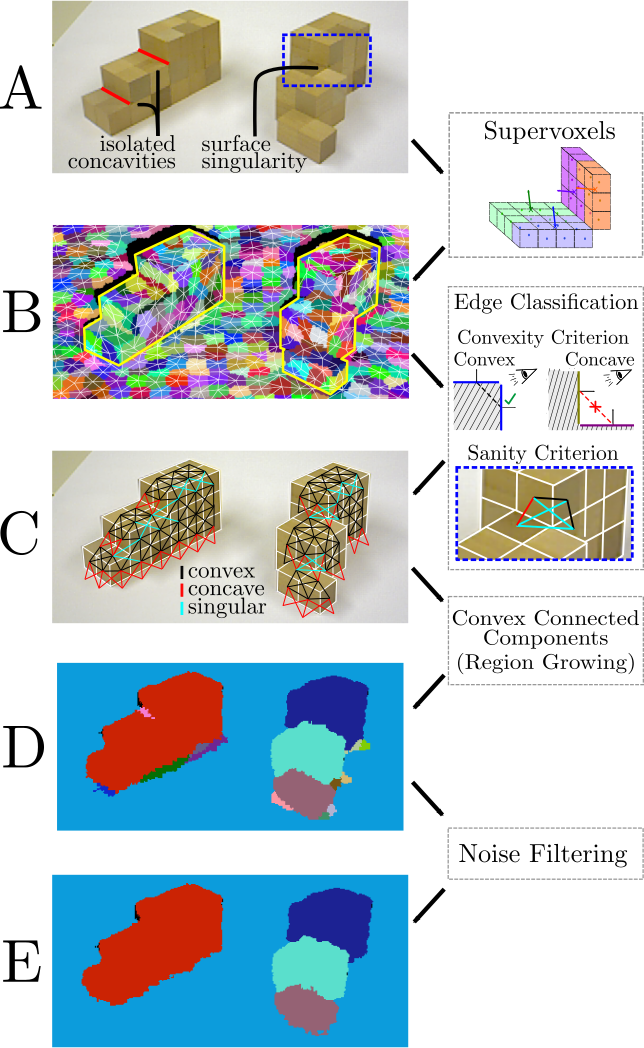
\includegraphics[width=0.7\linewidth]{figures/CVPR2014/flow_diagram}
    \caption[Flow Diagram of LCCP]{Flow diagram of the segmentation algorithm. \textbf{A)} RGB images corresponding to the point clouds of the scene. The red lines show two isolated concavities. The blue box shows an area with a surface singularity. \textbf{B)} Supervoxel adjacency graph. \textbf{C)} Model depicting the classified graph. Black lines denote convex connections, red lines concave ones and turquois lines singular connections (those, where two patches are connected only in a single point). \textbf{D)} Segmentation result; object labels are shown by different colors. \textbf{E)} Final result after noise filtering. The right column illustrates the supervoxel patches and the convexity and sanity criteria used for edge classification.}
  \label{fig:flow}
\end{figure}

As an example of an application of supervoxels and the adjacency octree, we shall briefly present a segmentation method which segments the supervoxel adjacency graph by classifying whether the connection $e=(\vec p_i, \vec p_j)$ between two supervoxels is convex (=valid) or concave (=invalid).

\textbf{Extended Convexity Criterion (CC)} Consider two adjacent supervoxels with centroids at the positions $\vec x_1,\vec x_2$ and normals $\vec n_1, \vec n_2$. Whether the connection between these is convex or concave can be inferred from the relation of the surface normals to the vector joining their centroids.

The angle of the normals to the vector $\vec d = \vec x_1-\vec x_2$ joining the centroids can be calculated using the identity for the dot product $\vec a\cdot \vec b = |\vec a|\cdot |\vec b|\cdot \cos(\alpha)$ with $\alpha = \measuredangle(\vec a,\vec b)$. For \textit{convex} connections, $\alpha_1$ is smaller than $\alpha_2$ (see Fig.~\ref{fig:details}~A). This can be expressed as:
  \begin{equation*}
    \alpha_1 < \alpha_2 \Rightarrow \cos(\alpha_1) - \cos(\alpha_2) > 0 \Leftrightarrow \vec {n_1}\cdot \hat d - \vec {n_2}\cdot \hat d > 0,
  \end{equation*}
where $\hat d = \frac{\vec{x_1}-\vec{x_2}}{||\vec{x_1}-\vec{x_2}||}$. Similarly, for a \textit{concave} connection we get:
  \begin{equation*}
    \alpha_1 > \alpha_2 \Leftrightarrow \vec {n_1}\cdot \hat d - \vec {n_2}\cdot \hat d < 0.
  \end{equation*}
Note that these operations are commutative, thus the choice of which patch is $\vec x_1$, does not change the result. Also the criterion is still valid if the $\vec x_i$ are displaced, as long as they stay within the surface.

To compensate for noise in the RGB-D data, a bias is introduced to treat concave connections with very similar normals, that is
\begin{align*}
  \beta = \measuredangle(\vec n_1,\vec n_2) = |\alpha_1-\alpha_2| = \cos^{-1}(\vec{n_1}\cdot \vec{n_2}) < \beta_\text{Thresh}~,
\end{align*}
as convex, since those usually represent flat surfaces. Depending on the value of the \textit{concavity tolerance threshold} $\beta_\text{Thresh}$, concave surfaces with low curvature are seen as convex and thus merged in the segmentation. This behavior may be desired to ignore small concavities. We set:
\begin{align}
  \text{CC}_b(\vec p_i, \vec p_j) :=
  \left\{\begin{array}{lc}
          \text{true} & \left(\vec {n_1} - \vec {n_2} \right) \cdot \hat d  > 0~ \lor~ (  \beta < \beta_\text{Thresh} )\\
            \text{false} & \text{otherwise.}\\
          \end{array} \right.
  \label{eqn:CC}
\end{align}

where the variable $CC_b$ defines the {\em basic convexity criterion}. However, local errors in the feature estimation caused by noise in the data can propagate very easily, potentially leading to errors in the resulting segmentation. This also makes the recognition of small concavities harder, as subtle features are more sensitive to noise. To improve on this we -- finally -- also include neighborhood information in the classification of edges: For a convex edge $e=(\vec p_i, \vec p_j)$, we require that there exists a common neighbor $\vec p_c$ of $\vec p_i$ and $\vec p_j$ that has a convex connection to both.

Thus we define \textit{extended convexity} $CC_e$:
\begin{align}
  \begin{aligned}
   \text{CC}_e (\vec p_i, \vec p_j) = \text{CC}_b(\vec p_i, \vec p_j) \land \text{CC}_b(\vec p_i, \vec p_c) \\ \land \text{CC}_b(\vec p_j, \vec p_c)
  \end{aligned}
\end{align}

With extended convexity, more evidence is necessary for a connection to be labeled as convex. Our implementation is based on the idea proposed by Moosmann \cite{Moosmann_Phdthesis}. In some cases results are already satisfactory even without using this type of neighborhood information. Thus, in the results section we will always denote whether this is used or not.\\

\begin{figure}[!ht]
 \centering
 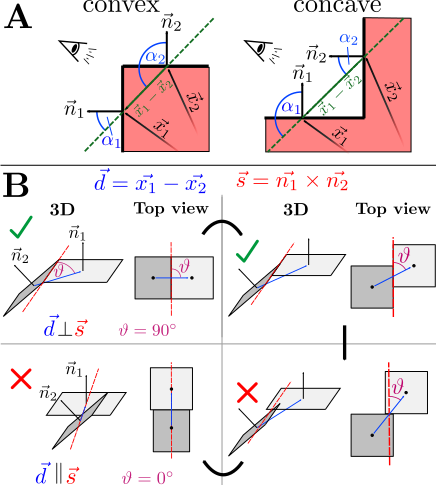
\includegraphics[width=0.7\linewidth]{figures/CVPR2014/algorithmic_details}
 \caption[Convexity Measures]{ \textbf{A)} Illustration of measures used in the basic convexity criterion. \textbf{B)} Illustration of the sanity criterion for decreasing values of $\vartheta$. Singular connections are characterized by small values of $\vartheta$.}
 \label{fig:details}
\end{figure}

\textbf{Region Growing:}
The second problem discussed in the Introduction, the danger of splitting objects along {\em isolated concavities}, can be addressed in the next step. For this we need to find all {\em clusters} of supervoxels, which belong to the same subgraph of valid convex connected edges. This is accomplished using a region growing process: First, an arbitrary seed supervoxel is chosen and labeled. This label is then propagated over the graph with a depth search that is only allowed to grow over convex edges. Once no new supervoxel can be assigned to the segment, we choose a new seed supervoxel that has not been labeled and propagate the new label as before, repeating the process until all supervoxels have been labeled. Note that all our criteria are commutative, so the output of the region growing does not depend on the choice of the seeds.\\



\section{Experimental Results}
\subsection{Datasets}
In the following sections we present quantitative results for VCCS and LCCP. We compare to state-of-the-art methods on the \textit{NYU Indoor Dataset}\cite{Silberman:ECCV12} and \textit{Object Segmentation Database}\cite{Richtsfeld:IROS12}. 

\subsubsection{Object Segmentation Database (OSD)}
The \textit{Object Segmentation Database} (OSD-v0.2) was proposed by Richtsfeld \textit{et al.}\cite{Richtsfeld:IROS12} in 2012. It consists of 111 cluttered scenes of objects on a table, taken with close proximity to the pictured objects. The scenes contain multiple objects, which have mostly box-like or cylindrical shape, with partial and full occlusions and heavy clutter in 2D as well as 3D. Importantly, most objects in the data set are \textit{simple}, that is, consist of only a single part. This makes the ground-truth data relatively non-ambiguous.

\begin{figure}[!ht]
 \centering
 \includegraphics[width=1\linewidth]{figures/CVPR2014/osd_examples}
 \caption[OSD Dataset Examples]{ Example results for the OSD dataset. Points beyond a distance of 2m were cropped for visualization. Parameters: $R_{voxel}=0.005$, $R_{seed}=0.02$, $\beta_\text{Thresh}=10^\circ$.  }
 \label{fig:OSD_results}
\end{figure}

The qualitative examples (Fig.~\ref{fig:OSD_results}) show that our algorithm performs very well in the segmentation of these cluttered scenes. The object separation can be intuitively understood: all objects present in the scenes are separated by concave boundaries, i.e. a line connecting neighboring surfaces of two different objects always travels through ``air''. This is also true for the boundary between an object and the supporting surface. As a consequence, objects that have a convex shape are correctly captured as one segment and separated from the other objects. Hollow objects (bowls, cups etc.) can be observed to show multiple segments inside, because the orientation of surface normals changes strongly on these concave surfaces. Despite most objects being simple, some objects have meaningful parts, such as handles or bottle caps, which are segmented by our algorithm.

The quantitative results (Table~\ref{tab:res_stat}) demonstrate that our approach is able to compete with state-of-the-art methods in the task of segmenting cluttered scenes with 'single-part' objects. Compared to the learning-based method from \cite{Richtsfeld:IROS12} we achieve better object separation ($F_{us}$), but higher oversegmentation error ($F_{os}$). The latter is because we sometimes detect object parts (\textit{e.g.} handles) and we do not utilize model fitting, which helps against noise. Comparing to the learning-free method of \"Uckermann \textit{et al.} \cite{Ritter2012} we obtain results within a standard deviation. Note that our actual goal is to partition complex objects into parts, which is dissimilar from the other two methods.

\begin{figure*}[!thb]
 \centering
 \includegraphics[width=1\linewidth]{figures/CVPR2014/nyu_examples.pdf}
 \caption[NYU Dataset Examples]{Example results for scenes from the NYU dataset using unsmoothed depth. Black areas indicate missing depth. Top row: rgb images. Mid. row: segmentation result. Bottom row: ground truth. Parameters A-C: $R_{voxel}=0.0075$, $R_{seed}=0.03$ and $\beta_\text{Thresh}=8^\circ$. Parameters D-E: $R_{voxel}=0.01$, $R_{seed}=0.04$ and $\beta_\text{Thresh}=10^\circ$ (identical to quantitative results, see Tab. \ref{tab:res_lccp_nyu}).}
 \label{fig:nyu_examples}
\end{figure*}

\subsubsection{NYU Indoor Dataset (NYU)}
The \textit{NYU Indoor Dataset}\footnote{\url{http://cs.nyu.edu/~silberman/datasets/nyu_depth_v2.html}} (NYUv2) from Silberman \textit{et al.}\cite{Silberman:ECCV12} is a large and complex dataset, consisting of 1449 cluttered indoor scenes. The data consists of pairs of aligned RGB and depth images, along with human annotated densely labeled ground truth. The images were captured in diverse indoor scenes, and present many difficulties for segmentation algorithms such as varied illumination and many small similarly colored objects. Examples of typical scenes are shown in Figure~\ref{fig:ExampleSegmentations}. One main difficulty presented by the dataset is that the distance to objects from the camera is quite large in the dataset. This results in significant depth quantization artifacts as well as few data points for many objects. Additionally, depth is often missing for extensive portions of many of the images, due to limitations of the Kinect sensor (e.g. reflective, transparent surfaces - windows are especially problematic). Silberman \textit{et al.} attempt to correct for these errors using a hole filling algorithm (smoothdepth), which estimates depth for missing areas based on the scheme from Levin \textit{et al.}\cite{Levin2004}.


\subsection {Supervoxels}
\label{sec:Evaluation}
In order to evaluate the quality of supervoxels generated by VCCS, we performed a quantitative comparison with three state-of-the-art superpixel methods using publicly available source code. 
We selected the two 2D techniques with the highest published performance from a recent review \cite{SLICCompared}: a graph based method, GCb10 \cite{SuperpixelsSupervoxels}\footnote{\url{http://www.csd.uwo.ca/~olga/Projects/superpixels.html}}, and a gradient ascent local clustering method, SLIC \cite{SLICCompared}\footnote{\url{http://ivrg.epfl.ch/supplementary_material/RK_SLICSuperpixels/index.html}}.
Additionally, we selected another method which uses depth images, DASP\cite{DASP}\footnote{\url{https://github.com/Danvil/dasp}}.
Examples of over-segmentations produced by the methods are given in Figure~\ref{fig:ExampleSegmentations}.
%------------------------------------------------------------------------
\begin{figure}[t]
\begin{center}
%\fbox{\rule{0pt}{2.4in} \rule{0.9\linewidth}{0pt}}
\includegraphics[width=0.9\linewidth]{figures/CVPR2013/BackTo2D.pdf}
\end{center}
   \caption[2D Hole Filling]{Example of hole-filling for images after returning from voxel-cloud to the projected image plane. Depth data, shown in the top left, has holes in it, shown as dark blue areas (here, due to the lamp interfering with the Kinect). The resulting supervoxels do not cover these holes as shown in the bottom left, since the cloud has no points in them. To generate a complete 2D segmentation, we fill these holes in using the SLIC algorithm, resulting in a complete segmentation, seen in the top right. The bottom right shows human annotated ground truth for the scene. }
\label{fig:ReturnToPlane}
\end{figure}
%------------------------------------------------------------------------

%------------------------------------------------------------------------
\begin{figure*}
\begin{center}
\includegraphics[width=1.01\linewidth]{figures/CVPR2013/Multiview.pdf}
\end{center}
   \caption[Supervoxels from Multiple Views]{Over-segmentation of a cloud from the RGB-D scenes dataset\cite{RGBDDataset}. The cloud is created by aligning 180 Kinect frames, examples of which are seen on the left side. The resulting cloud has over 3 million points, which reduces to 450k points at ${R}_{voxel}=0.01m$ and 100k points with ${R}_{voxel}=0.02m$. Over-segmentation of these take 6 and 1.5 seconds, respectively (including voxelization).}
\label{fig:MultiViewCloud}
\end{figure*}
%------------------------------------------------------------------------

%------------------------------------------------------------------------
\begin{figure*}
\begin{center}
\includegraphics[width=1.01\linewidth]{figures/CVPR2013/Comparison_Segmentation_Small.pdf}
\end{center}
   \caption[Superpixel Comparison]{Examples of under-segmentation output. From left to right- ground truth annotation, SLIC, GCb10, DASP, and VCCS. Each is shown with two different superpixel densities.}
\label{fig:ExampleSegmentations}
\end{figure*}
%------------------------------------------------------------------------

\subsubsection{Returning to the Projected Plane}
RGB+D sensors produce what is known as an organized point cloud- a cloud where every point corresponds to a pixel in the original RGB and depth images. When such a cloud is voxelized, it necessarily loses this correspondence, and becomes an unstructured cloud which no longer has any direct relationship back to the 2D projected plane. As such, in order to compare results with existing 2D methods we were forced to devise a scheme to apply supervoxel labels to the original image. 

To do this, we take every point in the original organized cloud and search for the nearest voxel in the voxelized representation. Unfortunately, since there are blank areas in the original depth image due to such factors as reflective surfaces, noise, and limited sensor range, this leaves us with some blank areas in the output labeled images. To overcome this, we fill in any large unlabeled areas using the SLIC algorithm. This is not a significant drawback, as the purpose of the algorithm is to form supervoxels in 3D space, not superpixels in the projected plane, and this hole-filling is only needed for comparison purposes. Additionally, the hole filling actually makes our results worse, since it does not consider depth, and therefore tends to bleed over some object boundaries that were correctly maintained in the supervoxel representation. An example of what the resulting segments look like before and after this procedure are shown in Figure~\ref{fig:ReturnToPlane}. 

%------------------------------------------------------------------------
\begin{figure}[t]
\begin{center}
%\includegraphics[width=0.8\linewidth,type=eps,ext=.eps,read=.eps]{Figures/boundary}
\includegraphics[width=0.95\linewidth]{figures/CVPR2013/Performance.pdf}
\end{center}
   \caption[Boundary Recall \& Undersegmentation Error]{Boundary recall and under-segmentation error for SLIC, GCb10, DASP, and VCCS.}
\label{fig:BoundaryRecall}
\label{fig:UndersegError}
\end{figure}
%------------------------------------------------------------------------
\subsubsection{Evaluation Metrics}
The most important property for superpixels is the ability to adhere to, and not cross, object boundaries. To measure this quantitatively, we have used two standard metrics for boundary adherence- boundary recall and under-segmentation error\cite{Turbopixels, SuperpixelsSupervoxels}. Boundary recall measures what fraction of the ground truth edges fall within at least two pixels of a superpixel boundary. High boundary recall indicates that the superpixels properly follow the edges of objects in the ground truth labeling. The results for boundary recall are given in Figure~\ref{fig:BoundaryRecall}. As can be seen, VCCS and SLIC have the best boundary recall performance, giving similar results as the number of superpixels in the segmentation varies. 

Under-segmentation error measures the amount of leakage across object boundaries. For a ground truth segmentation with regions $g_1,...,g_M$, and the set of superpixels from an over-segmentation, $s_1,...s_K$, under-segmentation error is defined as 
\begin{equation}
\label{eqn:UndersegError}
{E}_{useg}=\frac{1}{N} \left[ \sum_{i=1}^{M}{\left(\sum_{s_j \mid s_j \cap g_i}{|s_j|}\right)-N} \right],
\end{equation}
where $s_j \mid s_j \cap g_i$ is the set of superpixels required to cover a ground truth label $g_i$, and $N$ is the number of labeled ground truth pixels. A lower value means that less superpixels violated ground truth borders by crossing over them. Figure~\ref{fig:UndersegError} compares the four algorithms, giving under-segmentation error for increasing superpixel counts. VCCS outperforms existing methods for all superpixel densities. 

\subsubsection{Time Performance}
As superpixels are used as a preprocessing step to reduce the complexity of segmentation, they should be computationally efficient so that they do not negatively impact overall performance. To quantify segmentation speed, we measured the time required for the methods on images of increasing size (for the 2D methods) and increasing number of voxels (for VCCS). All measurements were recorded on an Intel Core i7 3.2Ghz processor, and are shown in Figure~\ref{fig:SegmentationSpeed}. VCCS shows performance competitive with SLIC and DASP (the two fastest superpixel methods in the literature) for voxel clouds of sizes which are typical for Kinect data at ${R}_{voxel}=0.008m$ (20-40k voxels). It should be noted that only VCCS takes advantage of multi-threading (for octree, kd-tree, and FPFH computation), as there are no publicly available multi-threaded implementations of the other algorithms.  

%------------------------------------------------------------------------
\begin{figure}[t]
\begin{center}
\includegraphics[width=0.95\linewidth]{figures/CVPR2013/Speed.pdf}
\end{center}
   \caption[Segmentation Speed]{Speed of segmentation for increasing image size and number of voxels. Use of GCb10 rapidly becomes unfeasible for larger image sizes, and so we do not adjust the axes to show its run-time. The variation seen in VCCS run-time is due to dependence on other factors, such as ${R}_{seed}$ and overall amount of connectivity in the adjacency graphs.}
\label{fig:SegmentationSpeed}
\end{figure}
%------------------------------------------------------------------------

\subsection{Locally Convex Connected Patches (LCCP)}

We compare segments against ground truth using three standard measures: \textit{Weighted Overlap} (WOv), which is a summary measure proposed by Silberman \textit{et al.} \cite{Silberman:ECCV12}, as well as \textit{false negative} ($fn$) and \textit{false positive} ($fp$) scores from \cite{Ritter2012} and \textit{over-} ($F_{os}$) and \textit{under-segmentation} ($F_{us}$) from \cite{Richtsfeld:IROS12}.

\begin{table*}[!htb]
  \centering
  \begin{tabular}{c|c|c|c}
%   \textbf{Overlap} & \textbf{Weighted Overlap} & \textbf{oversegmentation} & \textbf{undersegmentation} \\
  Method & Learned Features & Depth Data  & WOv\\ \hline \hline
  \multirow{2}{*}{LCCP} & NO LEARNING & depth & 53.6\% \\ \cline{2-4}
                                           & NO LEARNING & smoothdepth & 53.8\% \\ \hline
  LCCP + ext. convexity & NO LEARNING & smoothdepth &  57.6\% \\ \hline \hline
  \multirow{4}{*}{Silberman \textit{et al.}\cite{Silberman:ECCV12}} & RGB  & - &  50.3\% \\ \cline{2-4}
                                           & Depth & both  & 53.7\% \\ \cline{2-4}
                                           & RGB-D & both  & 60.1\% \\ \cline{2-4}
                                           & RGB-D + Support + Structure classes & both & 61.1\% \\ \hline \hline
  \multirow{2}{*}{Gupta \textit{et al.}\cite{Gupta:CVPR2013}} & gPb-ucm Gradients (from \cite{Arbelaez:PAMI2011}) & - &  55.0\% \\ \cline{2-4}
                                           & gPb-ucm + Depth + Concavity Gradients & both & 62.0\% \\ \hline
  \end{tabular}
  \caption[Comparison of NYU Dataset Results]{Comparison of different segmentation methods on the NYU dataset using weighted overlap \textit{WOv}. LCCP results were produced with voxel size $R_{voxel} = 0.01$, seed size $R_{seed}=0.04$ and concavity tolerance angle $\beta_\text{Tresh}=10^\circ$.}
  \label{tab:res_lccp_nyu}
\end{table*}

Example scenes in Fig.~\ref{fig:nyu_examples} show that the general object separation is still very good, which is expected from the results presented in the previous section. In contrast to the simple objects from the OSD dataset, however, in the NYU dataset the objects of interest are complex objects from various aspects of everyday life. As a consequence, these are mostly composed of multiple parts and thus our algorithm reveals interesting partitions. To give a few examples: In scene (A) the cupboard is partitioned into the top plate and its various drawers and the toilet is segmented into the flushing tank, the seat and the base. Scene (B) presents how a human is partitioned into hand, arm-bed, upper/lower part of the body and legs. For the sofas in scene (D) we get the two arm-rests, the back-rest and the seating. Note that in these cases the segments represent ``nameable regions'', which is also the case for many other segments (we discuss this further in Section~\ref{sec:nameable_parts}). It is evident that the ground truth data will then disagree with our labeling, which results in unjustified errors. For example, in scene (A) the ground truth considers the sink to be an important part, while the drawers are not labeled individually. Despite this disagreement, we do not consider either of the labelings wrong in general, but see them as different views on the data which are in many cases equally justifiable.

Because we designed our algorithm to detect object parts defined only by geometry, very thin objects like the posters on the background wall in scene (C) are not recognizable. Also the challenging data quality sometimes leads the part partitioning to fail, as seen for the human in scene (E). To show how well the general idea of part partitioning using concave boundaries works, we present results for a complex object with high data quality in the next section.

The quantitative results (Table~\ref{tab:res_lccp_nyu})\footnote{Updated results for \cite{Silberman:ECCV12} are available at \url{http://cs.nyu.edu/~silberman/datasets/nyu_depth_v2.html}.} show that our algorithm is able to produce good results on the challenging dataset. Despite being much simpler and without requiring learning on human annotated ground-truth, we compete with the approach from \cite{Silberman:ECCV12} when only depth information is used. Additionally, we still achieve 93\% of their score when comparing against the more complex feature spaces used in conjunction with learning-based algorithms. We should emphasize that our competitors do not aim for object parts but rather for ``whole object'' detections, specifically, those whole objects learned from this particular annotated ground truth. Conversely, our method establishes a general rule for object-ness that does not depend on this particular dataset, nor on the whims of a particular human annotator.

\section{Sequential Update of Perceptual Model}
Adding newly observed points to an existing supervoxel octree is accomplished through a three stage process. First, we must insert the points into the octree, and initialize new leaves for them if they did not exist previously. This results in an octree where leaves fall into three possible categories (illustrated in Fig.~\ref{fig:VoxelVisibility}; they are either new, observed, or unobserved in the most recent observation. Handling of new leaves is straightforward; we simply calculate adjacency relations to existing leaves and flag them as unlabeled. 
\begin{figure}[tb]
  \centering
  \includegraphics[scale=1.2]{figures/IROS2013/VoxelVisibility.pdf}
  \caption[Voxel Visibility]{Categorization of voxels based on new frame of data. Voxels fall into three categories, they are either new, observed or not observed in the frame. Furthermore, observed voxels can either have changed or remained the same, while voxels not observed in the frame are either occluded or no longer exist (in which case they should be deleted).}
  \label{fig:VoxelVisibility}
\end{figure}

To determine whether a leaf which existed previously has changed, we test the distance between the centroid of the points falling within its voxel (from the new frame) and its previous centroid. This is done in the same feature space used for growing the supervoxels, that is, we test whether the normal, color, and spatial location have varied more than a threshold value. This threshold is set to a relatively low constant value so that it favors false-positives (finding change when there was none), as they do not impact the tracking performance of the algorithm, but only have a slight effect on its run-time.  If a leaf is found to have changed, we remove its previous labeling. We also perform a global check to see if more than half of a supervoxels support has changed; if so, we completely remove the supervoxels label from all of its constituent voxels. 

Finally, we must consider how to handle leaves which were not observed in the inserted point cloud. Rather than simply prune them, we first check if it was possible to observe them from the viewpoint of the sensor which generated the input cloud. This occlusion check can be accomplished efficiently using the octree by determining if any voxels exist between unobserved leaves and the sensor viewpoint. If a clear line of sight exists from the leaf to the camera, it can safely be deleted. Conversely, if the path is obstructed, we "freeze" the leaf, meaning that it will remain constant until it is either observed or passes the line of sight test in a future frame (in which case, it can be safely deleted). This occlusion testing means that tracking of occluded objects is trivial, as occluded voxels remain in the observations which are used for tracking.

Once the octree voxels have been updated, we then proceed to update the supervoxels as before. That is, first we generate new seeds in regions of large unlabeled voxels, and then conduct the iterative region growing. This results in new supervoxels in regions which are new or changing, while leaving supervoxels in static and occluded regions unchanged. This reduces the tracking and segmentation problem to finding the best joint association of these new supervoxels with those from the prior time-step.

\section{Discussion}

In this Chapter we have presented several new concepts- the octree adjacency graph, supervoxels, a segmentation method which uses supervoxels, as well as a way to sequentially update an octree with new frames of data. Additionally, we have presented quantitative and qualitative results which demonstrate the usefulness of these techniques. In particular, LCCP has demonstrated the usefulness of a patch-based adjacency-graph interpretation of 3D Point Cloud data. We believe the results we achieved stem from two core properties: the ability of supervoxels to efficiently encode local regions, and the usefulness of a 3D adjacency-graph in resolving situations which are ambiguous in a 2D representation.

%% Requires fltpage2 package
%%
% \begin{FPfigure}
% \includegraphics[width=\textwidth]{figures/fullpage}
% \caption[Short figure name.]{This is a full page figure using the FPfigure command. It takes up the whole page and the caption appears on the preceding page. Its useful for large figures. Harvard's rules about full page figures are tricky, but you don't have to worry about it because we took care of it for you. For example, the full figure is supposed to have a title in the same style as the caption but without the actual caption. The caption is supposed to appear alone on the preceding page with no other text. You do't have to worry about any of that. We have modified the fltpage package to make it work. This is a lengthy caption and it clearly would not fit on the same page as the figure. Note that you should only use the FPfigure command in instances where the figure really is too large. If the figure is small enough to fit by the caption than it does not produce the desired effect. Good luck with your thesis. I have to keep writing this to make the caption really long. LaTex is a lot of fun. You will enjoy working with it. Good luck on your post doctoral life! I am looking forward to mine. \label{fig:myFullPageFigure}}
% \end{FPfigure}
% \afterpage{\clearpage}

\begin{savequote}[75mm]
Some Quote.
\qauthor{Quoteauthor Lastname}
\end{savequote}

%For an example of a full page figure, see Fig.~\ref{fig:myFullPageFigure}.
\chapter{Model-Based Point Cloud Tracking}
\label{Chap:ModelBasedTracking}
\lettrine[lines=3, loversize=0.3]{\textcolor{DarkBlue}T}{here's something to be said} for having a good opening line. 

\section{Particle Filters in 3D}
\section{Model Representation}
\section{Measurement Model}
\section{Dynamic Model}
\section{KL-Divergence Adaptation}
\section{Stratified Correspondence Sampling}
\todo[inline]{Provide simple experiment showing quality of track (maybe on VR Data) vs number of samples and particles.}
\todo[inline]{Also show result with occlusion? With some pure random samples added in?}
\section{Results on Virtual-Reality Data}
\begin{figure*}[!ht]
  \centering
  \includegraphics[width=\linewidth]{figures/Tracking/CombinedNoNoise.pdf}
  \caption[Tracked Output vs Ground Truth Artificial Sequence]{Tracked Output vs Ground Truth Artificial Sequence. The top panel shows position in terms of XYZ displacement and the bottom shows rotation in terms of geodesic. The location is generally tracked quite well, while the rotation is noisy due to the rotational symmetry of the two tracked objects (a bolt-angular and shaft).}
  \label{fig:CombinedNoNoise}
\end{figure*}

\begin{figure*}[!ht]
  \centering
  \includegraphics[width=\linewidth]{figures/Tracking/Action_Segmentation.pdf}
  \caption[Segmentation of Actions]{Segmentation of Cranfield Sequence into Keyframes - Tracked objects are monitored for when interactions between them occur, yielding keyframes which correspond to semantically important frames. Results here are shown for an artificial sequence with depth and RGB noise added.}
  \label{fig:ActionSegmentation}
\end{figure*}

\section{Results on Real Data}




\begin{savequote}[75mm]
Problems worthy

of attack

prove their worth

by hitting back. 
\qauthor{Piet Hein}
\end{savequote}

%For an example of a full page figure, see Fig.~\ref{fig:myFullPageFigure}.

\chapter{Tracking Based Point Cloud Video Segmentation}
\label{Chap:TrackingBasedSegmentation}
\lettrine[lines=3, loversize=0.3]{\textcolor{DarkBlue}S}{o far, we have presented} a 2D particle-filter based VOS method, developed a 3D point-cloud based world-model, and shown how it is possible to efficiently track within this model using particle filters. What remains is to bridge the gap between the tracked model results presented in the previous Chapter and the supervoxel representation of observations presented in the preceding one. There are many avenues available to proceed in doing this, and which one is optimal remains an open question. In this Chapter we shall describe the avenue which we pursued, show our results, and discuss where future research should lead.

Before we begin, it will probably be helpful if we show visually exactly what we are trying to achieve. Figure \ref{fig:TODOFIGURE} gives such an outline; the core idea is that we want to have a full segmentation of each frame.  While the tracking we have presented estimates a 6DoF pose for models in each frame, we now want to label every observed voxel (or supervoxel - which amounts to the same thing). Moreover, we want to use tracking as the basis for this labeling, due to its ability to maintain object identities through occlusions, sudden movements, and other difficult situations. 

\todo[inline]{Figure showing supervoxels, tracked models, associations to achieve segmentation}


\section{Tracked Model Representation}
The first issue that must be addressed is deciding at what ``level'' tracking should be done - at an object level, or at the supervoxel level. While ideally one could directly track supervoxels themselves, this is generally not feasible due to the aperture problem seen in neural visual fields~\cite{MarrApertureProblem}; local motion can only be estimated perpendicular to a contour that extends beyond its field of view~\cite{shimojo1989}. This means that in order to properly estimate motion of supervoxels, we must extend the field of view considered significantly beyond the size of the supervoxel itself; in fact, our aperture must contain the borders of the moving object in question, otherwise pairwise association of supervoxels is generally indeterminate. 

\todo[inline]{Figure showing aperture problem?}

As such, we must track higher level groupings - either objects or object parts. For the experiments we present later in this chapter, we initialize tracked models using a simple plane fitting and removal algorithm to remove supporting surfaces, followed by a euclidean clustering \cite{Radu3dIsHere} of the remaining supervoxels. This was done to simplify the experiments, though we should stress that any clustering method could be used to initialize the tracked object models, and indeed, one avenue of current research is using the LCCP segmentation presented in Chapter \ref{Chap:WorldModel} to initialize (and perhaps re-initialize) the models. In any case, regardless of the segmentation used, the supervoxel clusters are used to initialize the models which will be tracked. 

Similar to the previous Chapter, models consists of clouds - though now we use supervoxels rather than voxels, as seen in Figure~\ref{fig:TODOFIGURE}. Other than this consideration, the models are essentially identical to those given in Equations \ref{eqn:point} and \ref{eqn:model}. Just as each voxel in those equations is an average of the many points contained within the voxel, now each supervoxel's centroid is the average of all the voxels it contains. The main difference between the two on a local level is that supervoxels are not uniform in shape. Because of this, an important component of the supervoxel-based model which is not considered in the voxel version is the supervoxel connectivity graph. Additionally, supervoxels also have the additional information provided by a label - this is particularly important for non-moving objects, whose supervoxel labels will generally not change.

\todo[inline]{Figure showing points, voxels, and supervoxels (with connectivity) in a model.}

\section{Supervoxel-Based Particle Filters}
Tracking of the segmented models is accomplished using a bank of the correspondence-based particle filters from the previous Chapter. As our models now consist of supervoxels, so too must our observations - thus we use the supervoxels produced using the persistent scheme discussed in Chapter~\ref{Chap:WorldModel}. The observation model measures distance in a feature space of spatial distance, normals, color (in HSV space), and labels. Weights of predicted states $\mathbf{x}^j_t = [d_x, d_y, d_z, \gamma, \beta, \alpha]$ are measured by associating supervoxels from the transformed models to the observed supervoxels nearest in space. Particles are then weighted by measuring total distance in feature space, just as in (\ref{eqn:distance}), with the addition of a binary label term,
\begin{equation}
  \label{eqn:dist_labels}
    W_L =  \begin{cases} 1, & L_p = L_{p^*} \\ 
                         \frac{N_k-1}{N_k}, & L_p \neq L_{p^*} 
           \end{cases} 
\end{equation}

which results in the augmented distance function

\begin{equation} \label{eqn:augmented_distance}
  \tilde{w}^j = \sum_{1}^{\eta} \frac{1}{1 + \frac {\mu \lVert \mathbf{p}^j_{xyz} - \mathbf{p}^*_{xyz} \rVert} {R_{voxel}} +  \frac{\lambda D_c(p^j_{RGB},p^*_{RGB})}{m} +   \epsilon \lVert \mathbf{p}^j_{n_x n_y n_z} - \mathbf{p}^*_{n_x n_y n_z} \rVert + \nu  W_L}.
\end{equation}

As before, we adopt the notation $p$ for the supervoxel and $p*$ for its corresponding supervoxel in the observation.

KLD sampling \cite{KLDParticleFilter} is used to dynamically adapt the number of particles to the certainty of predictions. As matching supervoxel labels gives a high certainty of a correct prediction, objects which are not moving, and therefore have static supervoxel labels, need very few particles for accurate tracking. The details of KLD sampling are beyond the scope of this work, but we refer the reader to \cite{KLDParticleFilter} for an in-depth description of their operation. Outside of KLD sampling and the differences in the measurement function noted above, the particle filters function just as described in the previous chapter. The end result at each time-step are independent predictions of 6DoF object state, allowing a transformation of the model roughly aligning it with the currently observed supervoxels.  

\section{Association by Joint Energy Minimization}
The additional step that we must take to extract a full segmentation (rather than only object tracks) is to associate the observed supervoxels to the predictions coming from the particle filters. Therefore we must solve the multiple target data association problem. This is accomplished using an energy minimization which seeks to find an optimal global association of supervoxels to predictions. To do this, we first create a list of all observed supervoxels which lie within a radius $R_{seed}$ of each predicted supervoxel coming from the particle filters (see Fig.~\ref{fig:Association}). Then we select all supervoxels which could only be associated with one possible object, associate them, and remove them from further consideration.

\begin{figure}[tb]
  \centering
  \includegraphics[scale=1.0]{figures/IROS2013/Association.pdf}
  \caption[Supervoxel Association]{Association of observed supervoxels with predicted model supervoxels using global energy.}
  \label{fig:Association}
\end{figure}

To associate the remaining observed supervoxels, we determine which objects are competing for them, and then find the predicted supervoxel from each object which lies closest to them in the feature space (using spatial location, normals, and color as in (\ref{augmented_distance})). We adopt a RANSAC-like approach, similar to \cite{EnergyBasedMultiModel}, to sample from the set of possible associations and determine a global association which best aligns the predictions to the observed supervoxels. Additionally, we use a weighted sampling strategy where the likelihood of assigning object $k$ as the label $L$ of supervoxel $p$ falls off with increasing distance from the object centroid $C_k$
\begin{equation}
 \label{eqn:WeightSampling}
 \mathcal{L}(L_p=k | C_k) = \frac{1}{C_k}.
\end{equation}

To score a set of assignments, we compute a global energy, given in~(\ref{eqn:Energy}). Each global label association $\mathcal{A}$ consists of local associations $a$ which assign an object label $k$ to each observed supervoxel $p$. The first summation term, $ \sum_{p}{\|p^*_k - p\|} $, measures error in feature space between the observed supervoxel and the closest supervoxel in its associated predicted object $p^*_k$. 

\begin{equation}
\label{eqn:Energy}
{E}_\mathcal{A} =\prod_{a\in\mathcal{A}}{\Delta_k} \left( \sum_{p}{\|p^*_k - p\|} + \lambda \sum_{(p,p')\in \mathcal{N} }\delta(L_p \not= L_{p'}) \right) 
\end{equation}

The second summation is a smoothing prior which considers the adjacency graph of observed supervoxels. For every observed supervoxel, we compare its assigned label $L_p$ to the label of all supervoxels $p'$ which lie within its adjacency neighborhood $\mathcal{N}$. We adopt the Potts model as in \cite{Boykov2001}, where $\delta(\dot)$ is 1 if the specified condition holds, and 0 otherwise, and $\lambda$ is a weighting coefficient which controls the importance given to spatial continuity of labels.

Finally, the multiplicative term $\prod_{a\in\mathcal{A}}{\Delta_k}$ controls for the expansion or contraction of object volumes through the number of observed supervoxels associated with them. $\Delta_k$ penalizes for changes in volume by increasing the energy for deviations from unity in the ratio of observed supervoxels assigned to an object $\hat{N}_k$ with the number in the object model itself $\hat{N}_k$, that is

\begin{equation}
\label{eqn:DeltaSVs}
\Delta_k = \left\{ 
  \begin{array}{l l}
    {\hat{N}_k}/{N_k} & \quad \text{if ${\hat{N}_k} \geq {{N}_k}$ }\\
    2 - {\hat{N}_k}/{N_k} & \quad \text{if $\hat{N}_k < {N}_k$}~. 
  \end{array} \right.  
\end{equation}

Once the energy arrives at a stable minimum, we extract the resulting association of observed supervoxels to predicted results, and use them to update the tracked models.

\begin{figure*}[!ht]
  \centering
  \includegraphics[width=\linewidth]{figures/IROS2013/TrajectoriesNew.pdf}
  \caption[Cranfield Tracking Results]{Result of tracking and segmentation on Cranfield scenario from different views. Here the tracks are shown as dots of the color of the tracked label for each timestep. Initial locations of the pegs are shown in the middle bottom frame as semi-transparent masks. Calculated orientation is shown for the red peg with a set of axes every second time-step; these axes show pose in a frame relative to the start. }
  \label{fig:Trajectories}
\end{figure*}

\section{Alignment and Update of Models}
The joint energy minimization results in a global association $\mathcal{A}$ which assigns observed supervoxels to tracked objects. In order to use this to update the object models, we determine a transform which aligns it to the internal representation stored by the particle filter. As an initial guess, we use the inverse of the predicted state, and then use an iterative closest point \cite{ICPChetverikov} procedure to refine the transform such that the set of observed supervoxels best aligns with the model prior. We then replace the model prior with the new observed supervoxels. 

As a final step, we use the refined transform to update the states of the particles. To do this, we shift each particle $x_i$ towards the refined state $\hat{x}$, weighting the importance given to the refined state by a constant factor $\epsilon$

\begin{equation}
\label{eqn:PFUpdate}
x'_{i \in L} = (1-\epsilon) x_i + \epsilon \hat{x}~.
\end{equation}

For this work, we found that an $\epsilon$ of $0.5$ effectively removes noise (jitter) introduced by the replacement of the tracked model. Additionally, we correct the internal motion model of the particle filters to correspond to the new updated state.

\section{Experimental Results}
In order to demonstrate the usefulness of the proposed method, in this Section we first provide results from two successful applications. Both applications use the Cranfield scenario \cite{collins1984development} as in the previous chapter. Figure~\ref{fig:Trajectories} show the results of tracking and segmentation (only the pegs are shown in Figure~\ref{fig:Trajectories} to avoid clutter) using our Cranfield pieces. It can be seen that the algorithm is able to successfully extract full segmentation throughout the video.

%%%%%%%%%%%%%%%%%%%%%%%%%%%%%%%%%%%%
\subsection{Imitation of Trajectories for Robot Manipulation}
\begin{figure}[!tb]
  \centering
  \includegraphics[scale=0.84]{figures/IROS2013/RobotImitation.pdf}
  \caption[Trajectory Imitation]{Kuka LWR arm imitating trajectory and pose learned from tracked human demonstration.}
  \label{fig:Imitation}
\end{figure}
The standard way of teaching robots to perform human-like actions is imitation learning, also called programming by demonstration \cite{Billard2008,Argall2009}. There are several ways to demonstrate movements: 1) recording movements in joint-space (joint angles) or target-space (Cartesian space) by ways of a motion capture device (requires putting markers on human body), 2) using kinaesthetic guidance (guiding a robot's movements by a human hand), or 3) via teleoperation (controlling a robot via joystick). The only way to obtain motion trajectories from human observation in a "non-invasive" procedure is by using stereo vision \cite{Hecht2009}, however, usually it is model based. The tracking algorithm we have presented here can be used as an alternative method to obtain motion trajectories (in Cartesian space) in a model-free way. 

To demonstrate this, we applied our tracking algorithm to obtain human motion trajectories in Cartesian space including orientation of manipulated object (in total six DoFs). We tested it using a recording of the Cranfield scenario where, first, we let a human demonstrate the action and then reproduced it using a KUKA Light Weight Robot (LWR) arm \cite{kuka}. Specifically, here we imitate a human putting the separator block on the pegs. To generate trajectories for the robot from human demonstrations, we used a modified version of Dynamic Movement Primitives \cite{Ijspeert2002,Ijspeert2013} (DMP) and learning method as described in \cite{Kulvicius2012}. We used Cartesian impedance control and, thus, generated six DMPs (three for motion of the end-effector in Cartesian space and three for orientation of the hand) based on trajectories obtained from the tracking algorithm. Here we used 100 equally spaced kernels with width $\sigma=0.05$ for each dimension (for more details please refer to \cite{Kulvicius2012}).
 As demonstrated in Fig.~\ref{fig:Imitation} and the supplementary video, trajectories obtained by the proposed tracking algorithm are sufficiently accurate to allow reproduction of the human motion.

%%%%%%%%%%%%%%%%%%%%%%%%%%%%%%%%%%%%

\subsection{Semantic Summaries of Actions}
\todo[inline]{Need to show results on Eren's action recordings instead, but how to show it makes a difference. Maybe use it to do object classification at the end based on what the tracked action was? Or just say we generate SECs without needing object models.}

A fundamental task for intelligent autonomous robots is the problem of encoding long chain manipulations in a generic way, for use in tasks such as learning and recognition. As a demonstration of the usefulness of the proposed tracking framework, we use a recently introduced novel Semantic Event Chain (SEC) approach \cite{Aksoy11} which converts each segmented scene to a graph: nodes represent segment (i.e. object) centers and edges indicate whether two objects touch each other or not. By using an exact graph matching technique the SEC framework discretizes the entire graph sequence into decisive main graphs. A new main graph is identified whenever a new node or edge is formed or an existing edge or node is deleted. Thus, each main graph represents a “key frame” in the manipulation sequence. Figure~\ref{fig:SECGraphs} shows a few detected sample key frames from the long Cranfield action. While the complete action has in total 1453 frames, the SEC representation reduces it to just 35 key frames, each of which represents a topological change in the scene.

\begin{figure*}[ht!]
  \centering
  \includegraphics[width=\linewidth]{figures/IROS2013/SECKF.pdf}
  \caption[Cranfield Key Frames]{A few example key frames extracted from the long Cranfield action. Numbered nodes represent interacting objects, while edges show touching relations between objects. Each keyframe represents a topological change in the scene - here we show 4 of the 35 keyframes.}
  \label{fig:SECGraphs}
\end{figure*}
\begin{savequote}[75mm]
Some Quote.
\qauthor{Quoteauthor Lastname}
\end{savequote}

%For an example of a full page figure, see Fig.~\ref{fig:myFullPageFigure}.

\chapter{Conclusions}
\label{Chap:Conclusions}
\lettrine[lines=3, loversize=0.3]{\textcolor{DarkBlue}T}{hroughout this work,}  we have had one goal in mind; to develop video segmentation which has the reliability of tracking methods. The primary reason for doing this was to ensure the temporal consistency of segments through extended video clips of, in particular, indoor assembly tasks. Difficulties presented in such videos include partial and full occlusions, sudden and fast displacements of objects, different objects with similar or identical appearance, and objects which cannot be segmented based on color. Additionally, assembly tasks require a high degree of precision, particularly when it comes to the relative pose of parts when they are interacting (e.g. putting a bolt in a hole).

Our intended application for the segmentation of such videos was the general bootstrapping of assembly task understanding. If one can correctly track objects and their parts through a task without a-priori knowledge, it should be possible to use this to teach a robotic system from scratch. Not only this, but if one is able to correctly track full 6 DoF pose throughout a human-demonstrated assembly task, it is possible to learn trajectories that a robot can  use to directly imitate effective motion paths.

\section{Summary of Contributions}
We began in chapter \ref{Chap:VideoSegRelaxation} by presenting a 2D VOS method that made use of our proposed methodology; to use tracking as the basis for video segmentation. In particular, we showed how particle filters, a class of Sequential Bayesian Monte Carlo methods, can be used to predict what the next frame's segmentation should look like. These proposed segment masks were then combined using a weighted sampling strategy and then refined to fit observed image data using a relaxation process.

Next, in chapter \ref{Chap:WorldModel} we introduced RGB-D sensors, how they can be used to produce 3D point cloud data, and how this data can be organized using an octree structure. We then presented a specialized type of octree - the adjacency octree - which we developed to allow quick and efficient traversal between neighboring voxels within the tree. We subsequently showed how the adjacency octree can be used to efficiently further sub-divide voxel data into localized patches, called supervoxels, using our Voxel Cloud Connectivity Segmentation (VCCS). The utility of supervoxels was then demonstrated by showing their effectiveness in segmenting static scenes using a local convexity criterion (LCCP). The effectiveness of VCCS and LCCP were then demonstrated by showing their favorable results on a large state-of-the-art benchmark as compared to other state-of-the-art methods. Finally, we conclude the chapter by presenting how an adjacency octree containing supervoxels can be sequentially updated with new frames of data without deleting potentially occluded voxels.

We then extended the particle filter framework in chapter \ref{Chap:ModelBasedTracking} to 3D point clouds by formalizing the notion of a voxel-based measurement and dynamic model. While this straightforward implementation worked, we showed how it could achieve much faster (real-time on standard hardware) run times and accuracy by sampling correspondences. This improvement was then quantified using artificial data generated using a virtual reality simulator. As a final demonstration of the effectiveness of the tracker, we presented results on recordings of humans constructing the Cranfield benchmark. This showed how the tracker can be used to distill semantic understanding from a video sequence. 

Finally, in chapter \ref{Chap:TrackingBasedSegmentation} we tackled the problem of extracting full segmentations from tracked results. To do this, we first showed how the 3D particle filter presented previously could be extended to work on supervoxels. Then we showed how the adjacency graph of supervoxels could be used along with a global energy minimization to resolve interactions between trackers and produce a full segmentation consistent with the tracked poses. As a final demonstration of the presented methodology, we give results on several recordings of manipulation actions. 

Another important contribution was the development of the open-source Oculus vision system discussed in Appendix~\ref{chap:Oculus}. This system served as the platform on which much research has been done over the past several years and was a key tool in publications by several other researchers. Finally, we would like to note that most of the algorithms discussed in this work have been released as open-source to the vision community as part of the Point Cloud Library \footnote{\url{http://www.pointclouds.org/}}. We consider both of these important contributions, as the open sharing of code is vital to the advancement of the discipline of Computer Science.

\section{Shortcomings of VOS Benchmarks}
Evaluation of segmentation algorithms is a notoriously vexing problem due to the inherent ambiguity of what constitutes a ``correct'' segmentation. As such, in our work we have determined that we should avoid making concrete decisions on segmenting objects in single works, and instead chose to limit ourself to the lower, supervoxel level. While this is not an entirely satisfactory solution, we felt that there is simply not enough information in a single frame to extract meaningful segmentations accurately. Indeed, one cannot really tell the granularity with which a scene should be segmented into distinct objects until they see some action.

Benchmarking of 3D point cloud segmentation is a young topic - in fact, the first extensive benchmark, the \textit{NYU Indoor Dataset}, was not published until 2012 \cite{Silberman:ECCV12}. As such, it has many complications (that did not exist in 2D) which have yet to be resolved, such as that it is difficult, if not impossible, to make a 2D ground truth annotation correctly line up with the 3D point cloud representation. Even more to the point, there are still no 3D VOS benchmarks. In fact, even though the field is decades old, one must look to 2013 to find a 2D VOS benchmark \cite{Galasso2013}. There are many reasons for this lack of a proper benchmark, but the primary one is that is simply extremely time consuming to annotate ground-truth for even very short video sequences. Furthermore, labeling a single ground truth is even more difficult for video than single images, for instance, what happens when one takes a cap off of a bottle; should it be given a new label? If so, should it have had a separate label the entire time, or only once it is separated? What happens when objects become occluded and then reappear; should they be given new identities or maintain their old ones? If they keep their old ones, how long should we allow an object to be occluded for before we ``forget'' it?

Due to all of these concerns, we have made the decision in this work to benchmark our video segmentations by evaluating their ability to properly recognize actions. This, combined with qualitative results, effectively show the effectiveness of the method without the need to haggle over inscrutable questions such as ``what constitutes an object''?

\section{Limitations and Direction of Future Work}
The main limitation of the 2D tracking framework presented in chapter \ref{Chap:VideoSegRelaxation} is that it can only ``guess'' at correct behavior when an object is occluded. Indeed, this is a general problem of trying to infer behavior in a 3D world from observations in a 2D projected plane. It is because of these ambiguities and an inability to resolve them in a comprehensive and satisfying manner that we proceeded to tracking in 3D using RGB+D observations.

While our persistent voxel world model is very effective at maintaining the existence of stationary objects through occlusions, it does not handle objects which move while they are occluded. Solving this problem at the low-level of voxels is an unresolved problem, the outlook of which is fairly bleak. Our attempts at solving the problem lead us to believe that higher level object knowledge is necessary to account for occluded motion. With this in mind we are investigating a way of associating occluded objects with their occluder so that they move with them. Another limitation which we are currently addressing is that our persistent voxel world model does not account for camera motion. There is some existing work on real-time camera pose estimation, and we are hoping to incorporate such a method into our system in the near future.

As with any VOS method, our final result has a few important limitations. One of these is the need to set a rate at which to allow models to change. In many cases, objects are rigid, and do not change; allowing them to change only adds instability to the segmented output. Conversely, some objects are deformable, or not entirely visible in the scene, and will need to change to be correctly segmented. Another limitation is that we currently have no mechanism for adding new objects to the scene without reinitializing the tracking. Our current work focuses on correcting both of these limitations by incorporating the results of LCCP segmentation into the global minimization process to allow for parameter-free changing of models as well as the automated initialization of new tracks.






%% Requires fltpage2 package
%%
% \begin{FPfigure}
% \includegraphics[width=\textwidth]{figures/fullpage}
% \caption[Short figure name.]{This is a full page figure using the FPfigure command. It takes up the whole page and the caption appears on the preceding page. Its useful for large figures. Harvard's rules about full page figures are tricky, but you don't have to worry about it because we took care of it for you. For example, the full figure is supposed to have a title in the same style as the caption but without the actual caption. The caption is supposed to appear alone on the preceding page with no other text. You do't have to worry about any of that. We have modified the fltpage package to make it work. This is a lengthy caption and it clearly would not fit on the same page as the figure. Note that you should only use the FPfigure command in instances where the figure really is too large. If the figure is small enough to fit by the caption than it does not produce the desired effect. Good luck with your thesis. I have to keep writing this to make the caption really long. LaTex is a lot of fun. You will enjoy working with it. Good luck on your post doctoral life! I am looking forward to mine. \label{fig:myFullPageFigure}}
% \end{FPfigure}
% \afterpage{\clearpage}



\singlespacing

% the back matter
\clearpage
\bibliography{IEEEabrv.bib,PaponRefs.bib,references.bib,IROS2013.bib,ECCV2012.bib,cvpr2014.bib,dmp.bib}
\addcontentsline{toc}{chapter}{References}
\bibliographystyle{plainnat}
%\include{endmatter/colophon}

\onehalfspacing

\begin{appendices}
%For an example of a full page figure, see Fig.~\ref{fig:myFullPageFigure}.

\chapter{The Oculus Vision System}

%For an example of a full page figure, see Fig.~\ref{fig:myFullPageFigure}.

\chapter{Sequential Bayesian Estimation}

Sequential Bayesian estimation refers to a class of approaches for estimating a varying unknown probability density function from a time series of noisy observations. These approaches use a state space representation, in which a state vector $\mathbf{x}_t$ describes the hidden state of a dynamic system. The goal is to estimate the posterior distribution of the state given all prior observations $\mathbf{z}$, i.e., $\mathit{p}(\mathbf{x}_t|\mathbf{z}_{1:t})$. This is accomplished using a two step recursion which first generates a hypothesis of the current state conditioned on the previous state and then performs a Bayes update using the new observation. These steps are known as the prediction and filtering steps, respectively. 

The prediction step estimates the current distribution given all prior observations, or
\begin{equation} \label{eqn:prior}
\mathit{p}(\mathbf{x}_t|\mathbf{z}_{1:t-1}) =  \int{ \mathit{p}(\mathbf{x}_t|\mathbf{x}_{t-1})\mathit{p}(\mathbf{x}_{t-1}|\mathbf{z}_{1:t-1}) \mathit{d}\mathbf{x}_{t-1}}. 
\end{equation}
This requires the specification of a stochastic \textit{dynamic model} to characterize the state transition density $\mathit{p}(\mathbf{x}_t|\mathbf{x}_{t-1})$:
\begin{equation} 
\mathbf{x}_t = \mathit{f}_t(\mathbf{x}_{t-1},\mathbf{v}_t) ,
\end{equation}
where $\mathbf{v}_t$ is the process noise. The dynamic model takes advantage of knowledge of the system to generate reliable predictions of how the state evolves independent of observations. 

The filtering step uses Bayes rule to update the predicted density by conditioning it on the new observation $\mathbf{z}_t$:
\begin{equation} \label{eqn:posterior}
\mathit{p}(\mathbf{x}_t|\mathbf{z}_{1:t}) =  \frac{ \mathit{p}(\mathbf{z}_t|\mathbf{x}_{t})\mathit{p}(\mathbf{x}_{t}|\mathbf{z}_{1:t-1})} {\mathit{p}(\mathbf{z}_{t}|\mathbf{z}_{1:t-1})}. 
\end{equation}
This requires the specification of a \textit{measurement model} to characterize the observation density $\mathit{p}(\mathbf{z}_t|\mathbf{x}_{t})$:
\begin{equation} 
\mathbf{z}_t = \mathit{h}_t(\mathbf{x}_{t},\mathbf{w}_t) ,
\end{equation}
where $\mathbf{w}_t$ is the measurement noise. The marginal likelihood $\mathit{p}(\mathbf{z}_{t}|\mathbf{z}_{1:t-1})$ is constant relative to the state, and is generally ignored in practice and replaced with a simple normalizing factor. 

Once the filtered, or posterior distribution is determined, an estimate of the state can be made using a variety of techniques (e.g., MAP, mean-shift). 

\section{Particle Filters}
Unfortunately, except for in special cases (such as the linear Gaussian case with the Kalman filter) determining an exact solution for the posterior distribution is not feasible. As such, Particle Filter techniques were developed to approximate the posterior distribution. They use sequential Monte Carlo to directly implement the Bayesian recursion equations on a set of samples. The most common Particle Filter algorithm is Sequential Importance Sampling (SIS) recursively updates a set of $N$ samples (particles) from the previous time step $\{ \mathbf{x}^{i}_{t-1}, w^i_{t-1} \}$ in a two-step procedure: 

\begin{enumerate}
 \item \textbf{Predict:} Apply the dynamic model to find an estimate of the new state for each particle, $\tilde{\mathbf{x}}^{1..N}_t$. That is, draw samples from the state transition prior distribution $\mathit{p}(\mathbf{x}_t|\mathbf{x}_{t-1})$.
 \item \textbf{Update:} Evaluate the weight for each particle using the observation density:  $\tilde{w}^i_t = \mathit{p}(\mathbf{z}_t|\tilde{\mathbf{x}}_{t})$ and then normalize.
\end{enumerate}

The set of weighted particles $\{ \mathbf{x}^{i}_{t}, w^i_{t} \}$ then approximates the posterior distribution, and an overall state estimate can be found using any appropriate method.

\subsection{Resampling}
An important issue with SIS is that for any finite number of particles the weights will tend to degenerate to the trivial set where all particles have weight zero except for one. This results in the observations having no effect on the particle trajectories, meaning the filter amounts to a random walk using the dynamic model. To avoid this problem, a resampling step was added \cite{GordonEtAlPf, Rubin:SIR} which generates a new particle set by sampling from the existing particle set. The simplest way of doing this is to simply sample from the multinomial distribution of the particle weights and then set all particle weights to $1/N$. While this \textit{multinomial resampling} can be effective if employed judiciously, it can also lead to other problems, namely an increasing variance of the posterior distribution. To overcome this a variety of low-variance resampling techniques have been developed; we refer the reader to \cite{Douce:Resampling} for a concise summary of the different approaches.



\end{appendices}

\end{document}
